\listfiles
\documentclass[12pt,a4paper]{article}
% encoding, language
\usepackage[T1]{fontenc}
\usepackage[utf8]{inputenc}
\usepackage[magyar]{babel}
\usepackage{fontspec}
\setmainfont{Times New Roman} 

% layout
\usepackage[margin=2cm]{geometry}
\usepackage{xcolor}
\usepackage[font=small,justification=centering, labelfont=bf]{caption}
\captionsetup[figure]{labelfont=bf}
\captionsetup[table]{labelfont=bf}

% math
\usepackage{amsmath, amssymb, amsfonts}
\usepackage{gensymb}
\numberwithin{equation}{section}

% figures
\usepackage{graphicx}
\usepackage{subcaption}
\usepackage{float}
\numberwithin{figure}{section}


% tables
\usepackage{multirow}
\usepackage{longtable}
\usepackage{multicol}
\numberwithin{table}{section}


% refs
\usepackage[colorlinks=true, linkcolor=blue, citecolor=blue, urlcolor=blue]{hyperref}
\usepackage{url}
\usepackage{csquotes}

%abstract
\addto\captionsmagyar{\renewcommand{\abstractname}{Absztrakt}}


\begin{document}

\begin{titlepage}
    \centering
    \vspace*{1cm}
    {\large Eötvös Loránd Tudományegyetem Természettudományi Kar\par}
    \vspace{0.5cm}
    {\Huge \bfseries Gépi tanuláson alapuló időjárás-előrejelző modell kaotikusságának vizsgálata légköri trajektóriákkal\par}
    \vspace{1cm}
    {\Large Tudományos Diákköri Konferencia dolgozat}
    
    \vspace{3cm}
    
\includegraphics[width=12cm]{elte_logo.png}
    \vspace{3cm}
    

    {\Large
    Készítette: \textbf{Opposits Ágota}\par}
    {\large Fizika BSc, meteorológus szakirány, III. évfolyam\par}
    \vspace{0.5cm}
    {\Large Témavezető: \textbf{Leelőssy Ádám} \par}
    {\large Egyetemi adjunktus\par}
    {\Large Témavezető: \textbf{Haszpra Tímea} \par}
    {\large Tudományos főmunkatárs\par}
    \vspace{1cm}
    {\Large Budapest, 2026 \par}
    
\end{titlepage}


\tableofcontents
\newpage

\begin{abstract}
    A mesterséges intelligencián alapuló időjárás-előrejelző modellek (Machine Learning Weather Prediction, MLWP) 2020-as évek elején történő elterjedése óta sok kutatás irányult a hagyományos előrejelző technológiáktól alapjaiban eltérő módszer adta lehetőségek vizsgálatára. A modern MLWP-modellek mély neurális hálózat alapúak, és egy költségfüggvény minimalizálására vannak betanítva. Az adatalapú megközelítés következtében a modellek nem ismerik expliciten a légkör kormányzó egyenleteit, amely fizikai inkonzisztenciákhoz vezethet. A szakirodalom jelenleg nem tekinti az MLWP-modelleket a légkör megfelelő szimulátorainak.

    Kutatásomban trajektóriamodellezésen keresztül megvizsgálom, hogy a European Centre for Medium-Range Weather Forecasts (ECMWF) jelenleg élvonalbeli hagyományos, kaotikus jegyeket bizonyítottan mutató modelljével (IFS) szemben az MLWP-modellje (AIFS) mutat-e kaotikus viselkedést.

    2026. június 1-jén UTC 0 órakor futtatott szélelőrejelzéseket használtam. Az előrejelzések tér- és időbeli felbontásának finomítása lineáris interpolációval történt. Egymáshoz közel indított részecskék trajektóriáira felírt, csak a szél sodrását figyelembe vevő differenciálegyenlet-rendszert adott izobárszinten a modellek szélsebesség-előrejelzéseit felhasználva numerikusan integráltam. A részecskéket összekötő fonal hosszának exponenciális időbeli változásából topologikus entrópia számolható.

    Az IFS és AIFS esetében is sikerült exponenciális időbeli változást kimutatni, és pozitív topologikus entrópiát meghatározni, ami kaotikus viselkedésre utal. Durva térbeli felbontáson topologikus entrópia nem volt meghatározható. 150 óránál hosszabb előrejelzési időtávon az exponenciális kapcsolat az IFS-nél és AIFS-nél is kimutathatatlanná vált, ami a szomszédos részecskék egymástól való túlzott eltávolodásával, ezáltal pedig a topologikus entrópia alulbecslésével magyarázható.
    A vizsgált szinteken (500, 700, 850 hPa) az AIFS topologikus entrópiája jellemzően alacsonyabb, mint az IFS-é, melynek oka lehet az MLWP modellekre jellemző elmosódás jelensége. A vizuálisan ábrázolt, IFS szélelőrejelzésén alapuló trajektória-előrejelzések AIFS-énél komplexebb térbeli szerkezete is ezt támasztja alá. A földfelszín zavaró hatása megfigyelhető, magasabb nyomású izobárszinteken a topologikus entrópia magasabb.

    Az alkalmazott lagrange-i megközelítés alapján tehát az AIFS is mutat kaotikus tulajdonságokat, ami azt jelenti, hogy a modell nem veszíti el teljesen a tanulás során a légkör ezen tulajdonságának reprezentálását, de az elmosódás hatása megfigyelhető.
\end{abstract}
\newpage

\section{Bevezetés}

\subsection{Célkitűzés}
A huszadik század eleje óta -- többek között a ,,bergeni iskola" neves kutatóinak köszönhetően -- ismerjük a légkör működését leíró nemlineáris egyenletrendszert, az úgynevezett kormányzó egyenleteket. Az időjárás-előrejelzés hagyományosan ezen egyenletrendszer integrálásán alapul, melyet szuperszámítógépeken futó numerikus modellek hajtanak végre (\textit{Numerical Weather Prediction, NWP}). Az utóbbi években jelentős áttörés történt az időjárás-előrejelzés területén: a 2020-as évek elején megjelentek a gépi tanulás alapú időjárás-előrejelző modellek (\textit{Machine Learning Weather Prediction, MLWP}). A gépi tanulás alapú modellek rekonstruált historikus időjárási adatokból -- úgynevezett reanalízis adatokból --, illetve operatív NWP-előrejelzésekből tanulják meg a légköri folyamatok mintázatait, és ezáltal képesek a kiinduló adatok -- a peremfeltételek -- ismeretében predikciót adni a jövő várható időjárására. Az eltérő megközelítés folytán több előny és hátrány is megjelenik a hagyományos NWP-modellekhez képest.

Az MLWP-modellek legnagyobb előnye, hogy rendkívül rövid idő alatt képesek előrejelzést készíteni, melyek pontossága összevethető a hagyományos modellekével. Az első ilyen jelentősebb modell, az NVIDIA FourCastNet 2022-es publikációjában szereplő adatok is ezt támasztják alá: a modell 2 másodperc alatt képes egyhetes időjárás-előrejelzést készíteni, pontossága pedig az egyik legjobb NWP-modell, a European Centre for Medium-Range Weather Forecasting (\textit{ECMWF}) IFS nevű modelljével összemérhető \cite{pathak_fourcastnet_2022}. A 2022 óta eltelt években sorra jelentek meg az MLWP-modellek (pl. Huawei Pangu-Weather, 2023; Google GraphCast, 2023; FuXi, 2023; FengWu, 2023; ECMWF-AIFS, 2024; illetve néhány ensemble modell: Google GenCast, 2024; ECMWF AIFS ENS, 2025), és a tapasztalatok egybehangzóak: az előrejelzések rendkívül gyorsak és pontosak, ami megfelelő indok arra, hogy a modelleket még tovább fejlesszék.


A további fejlesztés mellett szól az adatalapú megközelítésből adódó alapvető hátulütők kiküszöbölésére való törekvés is. Egyik ilyen abból ered, hogy a modellek gyakran valamilyen négyzetes hiba, mint a négyzetes középhiba (\textit{Mean Squared Error, MSE}) alapú költségfüggvény minimalizálására vannak betanítva. Ennek következtében igyekeznek elkerülni a szélsőséges értékek predikcióját, mivel tévesen megállapított kiugró érték jelentős büntetést eredményezne. Az ilyen módon előálló szélsőérték-kerülést nevezzük ,,smoothing"-nak, utalva arra, hogy a kiugró csúcsok mintegy elmosásra kerülnek. 

Másrészt -- mivel a modell nem ismeri a légköri kormányzó egyenleteket, hanem csak korábbi időjárási adatok mintázataiból tanul -- elvileg lehetséges a fizikai valósággal inkonzisztens előrejelzés készítése is. Ilyen volt pl. az ECMWF-AIFS egy korábbi verziójának az a hibája, hogy negatív csapadékmennyiséget jelzett előre. A modellfejlesztők a valósághű predikciókat elérendő fizikai kényszerfeltételek bevezetésével korlátozzák a modellt \cite{moldovan_update_2025}. 

Többek között a fentebb említett hibák miatt a szakirodalom jelenleg nem tekinti az MLWP modelleket a légkör megfelelő szimulátorainak \cite{bonavita_limitations_2024}. A szakirodalomban azonban még nem sok kutatás tűzte ki céljául a gépi tanulás alapú időjárás-előrejelző modellek kaotikus tulajdonságainak vizsgálatát. Kutatásomban azt szeretném megvizsgálni, hogy a fizikai törvények helyett adatokon alapuló megközelítés kimutathatatlanná teszi-e az előrejelzésekben a légkör egy alapvető tulajdonságát, a káoszt. Amennyiben a modellek nem tudják reprodukálni a kaotikus jegyeket, úgy hamis biztosságot adhatnak a hosszú távú előrejelzések megbízhatóságára \cite{selz_can_2023}. Ha azonban észlelhető a káosz a modell előrejelzéseiben, az azt jelenti, hogy az adatalapú tanítás következtében mégsem vész el minden fizikai törvényszerűség.

\subsection{A mesterséges intelligencia és gépi tanulás}

A mesterséges intelligencia fogalmát John McCarthy, Marvin Minsky, Claude Shannon és Nathaniel Rochester alkották meg 1956-ban a Dartmouth workshop-on (\textit{Dartmouth Summer Research Project on Artificial Intelligence}). Felvetett elvük azon alapult, hogy ,,a tanulás minden aspektusa, vagy az intelligencia bármely más jellemzője elvileg olyan pontosan leírható, hogy egy géppel azt szimulálni lehet" \cite{moor_dartmouth_2006,choi_introduction_2020}. A tanulás általános fogalma új ismeretek, képességek és viselkedésminták elsajátítását vagy módosítását jelenti. A mintázatok megismerése által lehetővé válik a jövőre vonatkozó előrejelzések készítése. Gépek esetében a tanuláshoz szükséges tapasztalatszerzés adatok alapján, mintázatfelismerés által történik; ezt nevezzük gépi tanulásnak \cite{alzubi_machine_2018}. 

Az első gépi tanulás alapú technológia az 1990-es években lett népszerű, amikor megjelentek az elektronikus levelezőrendszerekben a spamfilterek: a szűrő felhasználói bejelentésekből származó adatokon lett betanítva, megtanulva, hogy milyen jellemzői vannak egy spam e-mailnek. Az ezt követő évtizedekben egyre több gépi tanulás alapú technológia jelent meg, gondolhatunk itt a mindennapokban gyakran használt beszédfelismerő eszközökre, vagy a közösségi média tartalomajánló algoritmusaira \cite{geron_hands-machine_2017}. A gépi tanulást 1959-ben Arthur Samuel amerikai informatikus így definiálta \cite{lee_machine_2017}: 
\begin{displayquote}
    \textit{A gépi tanulás képessé teszi a számítógépeket a tanulásra anélkül, hogy explicit módon programoznánk őket.} 
\end{displayquote}
Egzaktabb definíciót nyújt Tom Mitchell szintén amerikai informatikus megfogalmazása \cite{mitchell_discipline_2006}: 
\begin{displayquote}
\textit{Egy számítógépes program valamilyen T feladat elvégzése érdekében -- melynek sikerességét valamely P teljesítményt értékelő mérőszám jellemzi -- E tapasztalatból tanul, ha a T elvégzése során nyújtott teljesítménye P mérőszámmal mérve az E tapasztalat megszerzésével javul.} 
\end{displayquote}
A gépi tanulás olyan problémák megoldásában lehet rendkívül hasznos, amik túl komplexek, vagy nem ismert algoritmikus megoldásuk. Ha megnézzük, hogy a gép milyen mintázatokat ismert fel vagy kapcsolatokat tanult meg, akkor az ember is új, addig még fel nem fedezett korrelációkat vehet észre, ami által a megértésünk javulhat, ezt nevezzük adatbányászatnak (\textit{data mining}). A példák, tapasztalatok, amik segítségével a gép tanul, a tanító adathalmaz (\textit{training set}) részét képezik (\textit{sample}) \cite{geron_hands-machine_2017}. 

A gépi tanulásos rendszereket csoportosíthatjuk aszerint, hogy humán felügyelet alatt van-e tanítva (felügyelt -- \textit{supervised}, felügyelet nélküli -- \textit{unsupervised}, félig felügyelt -- \textit{semisupervised}, megerősítéses -- \textit{reinforcement} tanulás); menet közben tud-e fokozatosan tanulni (\textit{online} és \textit{batch} tanulás); illetve hogy az új adatokat a már ismertekhez hasonlítja (példa alapú -- \textit{instance-based} tanulás) vagy a tanító adathalmazban mintázatokat ismer fel, és ez alapján előrejelzést tud adni (modell alapú -- \textit{model-based} tanulás). A legfontosabb fogalmak a fentiek közül a felügyelt, felügyelet nélküli, illetve megerősítéses tanulás \cite{geron_hands-machine_2017}. 

A felügyelt tanulás során a tanító adathalmaz tartalmazza a kívánt kimenetet / helyes megoldást (ezt nevezzük címkének -- \textit{label}). Példa lehet erre, hogy szeretnénk betanítani egy modellt, hogy korábbi eladási adatokat ismerve jelezze előre, mennyit ér egy eladásra szánt autó. Az autónak a tulajdonságai (\textit{feature}; mint a kora, megtett km, márka stb.) adottak. Az előrejelezni kívánt numerikus mennyiséget hívjuk \textit{predictor}-nek vagy \textit{target}-nek (jelen esetben ez az autó ára). Az előrejelzéshez használt algoritmus többféle lehet, legismertebb példái a lineáris regresszió és a neurális hálózat architektúrák. Felügyelet nélküli tanulás során a tanító adathalmaz nincsen felcímkézve, a modell maga tanulja meg a jellemzőket elkülöníteni. Legismertebb példa a klaszterezés (\textit{clustering}), amikor a modell a vizsgált adatokat a megfigyelt tulajdonságaik alapján osztályozza. Megerősítéses tanulás esetén a tanuló rendszer (az ágens -- \textit{agent}) megfigyeli a környezetét és a kialakított irányelvének (\textit{policy}) megfelelően tetteket hajt végre. A tetteiért jutalmat (\textit{reward}) vagy büntetést (\textit{penalty}) kap. Az ágens célja a jutalom maximalizálása, ami érdekében iteratívan frissíti az irányelvét \cite{geron_hands-machine_2017}. 

A gépi tanulás alapú modellek problémái legtöbbször a tanító adatból származnak: gondot jelent a nem megfelelő mennyiségű, minőségű, nem elég reprezentatív, vagy irreleváns adat. Ha a modell túl komplex a feladathoz, felléphet a túlillesztés (\textit{overfitting}), ami azt jelenti, hogy az illesztett függvény helytelenül a zajt is figyelembe vette. Ha a modell túl egyszerű, azt alulillesztésnek (\textit{underfitting}) nevezzük. Az elkészült gépi tanulás alapú modelleket ezen hibák kiszűrése érdekében validálják, melynek népszerű eszköze az igazságmátrix (\textit{confusion matrix}) \cite{geron_hands-machine_2017}.

A gépi tanulás hagyományosan statisztikai módszerek segítségével történik a megfigyelt adatok alapján. A gépi tanulás múlt században megalkotott, és az utóbbi évtizedekben elterjedt technikája egészen más megközelítést kínál; ezek a mesterséges neurális hálózatok (\textit{Artificial Neural Network, ANN}). Az ANN-ek segítségével az adatbázisban fennálló komplex kapcsolatok is felismerhetőek \cite{sharifani_machine_2023}. Az ANN-eket 1943-ban mutatta be Warren McCulloch amerikai neurofiziológus és Walter Pitts számítógépes idegtudós. Az ANN-t mesterséges neuronok alkotják, melyek működését a biológiai neuronok ihlették, melyet az \ref{fig:bio_neur}. ábra mutat be.

\begin{figure}[H]
    \centering
    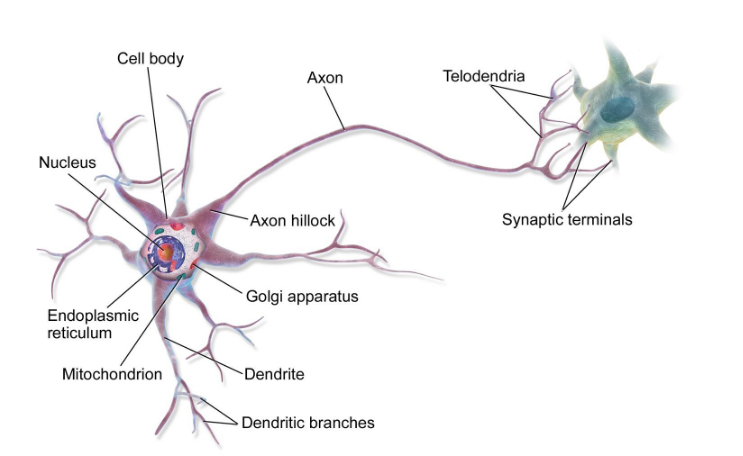
\includegraphics[width=0.5\linewidth]{../figures/bio_neur.png}
    \caption{A biológiai neuron szerkezete. Az ábra Géron \textit{Hands-On Machine Learning with Scikit-Learn and TensorFlow} (2017) \cite{geron_hands-machine_2017} könyvéből származik.}
    \label{fig:bio_neur}
\end{figure}

A biológiai neuron (idegsejt) az agykéregben előforduló sejt, melynek főbb részei a sejttest (\textit{cell body}), a dendritek (\textit{dendrite}), illetve a nagyon hosszú nyúlványa, az axon. Az axon telodendronokra bomlik, melyek csúcsán kis szinapszisok találhatóak, melyek a dendritekbe tudnak kapcsolódni és a neuronok kis elektromos impulzusokkal történő kommunikációjáért felelősek. Ha a neuron adott idő alatt elég jelet kap, maga is aktiválódik és jeleket ad le. A biológiai neuronok közti kapcsolódási pont a szinapszis, ami erősödik, ha a két neuron gyakran aktiválódik együtt \cite{choi_introduction_2020}. Az agyban a neuronok egymás utáni rétegekbe vannak rendeződve, így lesz képes az emberi agy komplex feladatok elvégzésére is \cite{geron_hands-machine_2017}.

Az ANN rétegebe rendeződött neuronokból áll. A rétegekben csomópontok vannak, az információ feldolgozásáért felelős mesterséges neuronok pedig kapcsolatokon keresztül kommunikálnak egymással \cite{sharkawy_principle_2020}. A csomópontok a biológiai neuron sejttestének feleltethetőek meg, a kapcsolatok pedig hasonlóan működnek, mint az axonok és dendritek. A mesterséges neuronok közti kapcsolat erősségét a súlyok (\textit{weight}) határozzák meg \cite{choi_introduction_2020}.

A McCulloch és Pitts által megalkotott ANN kijelentéslogikán alapult. A neuronok egy vagy több bináris (\textit{on/off} típusú) bemenetet (\textit{input}) fogadtak, és egyetlen kimenetet (\textit{output}) adtak. A biológiai neuronok aktiválódását úgy imitálták, hogy a mesterséges neuron csak akkor adott kimenetet, ha a kapott bemenetek száma elért egy bizonyos értéket. 

Az egyik legegyszerűbb neurális hálózat a Perceptron, melyet 1957-ben Frank Rosenblatt mutatott be. Úgynevezett küszöb logikai egységek (\textit{Treshold Logic Unit, TLU}) a mesterséges neuronok, az input és output értékek pedig numerikusak; minden input -- fontosságának megfelelően -- súlyozva van. A súlyozott bemenetek mellett egy $b$ konstans értéket felvevő elfogultság (\textit{bias}) is hozzáadásra szokott kerülni. A TLU egy súlyozott összeget számol, majd egy nemlineáris aktivációs függvényt hattat az eredményre, és ezt adja outputnak. Az aktivációs függvényre azért van szükség, hogy a lineárisnál bonyolultabb kapcsolatokat is képes legyen megtanulni az ANN. Aktivációs függvény lehet pl. a Heaviside-féle egységfüggvény, ReLu (\textit{REctified Linear Unit}, ami a negatív értékeket lenullázza), de gyakran valamilyen szigmoid függvényt alkalmaznak a célra, mint a tangens hiperbolikusz vagy a logisztikus függvény. A mesterséges neuron működését az alábbi egyenlet foglalja össze:
\[
s_j=\sum_{i=1}^m w_{ij}\cdot x_i + b_j; \quad \hat{y_j}=\varphi(s_j),
\] 
ahol $x_i$ az input, $b_j$ a bias, $w_{ij}$ a súlymátrix, $s_j$ a súlyozott összeg, $\varphi$ az aktivációs függvény, $\hat{y_j}$ pedig az output. A fentebb leírt mesterséges neuron működését mutatja be a \ref{fig:perceptron}. ábra. \cite{sharkawy_principle_2020,geron_hands-machine_2017,kelleher_deep_2019}.

\begin{figure}[H]
    \centering
    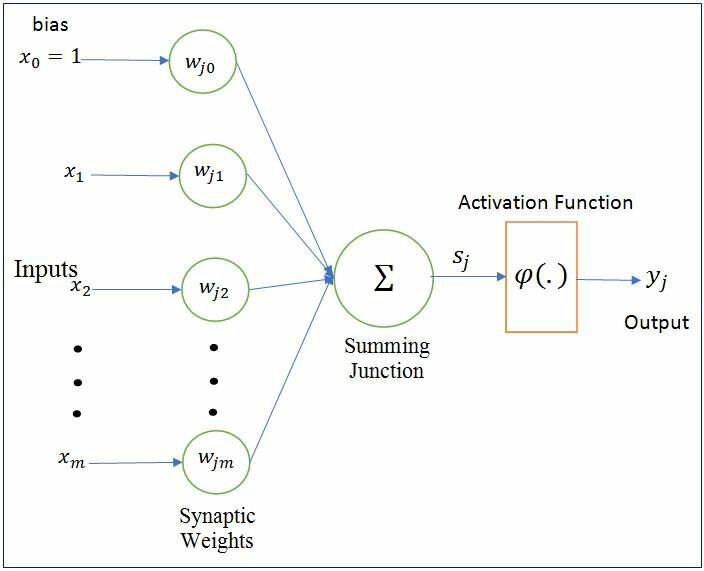
\includegraphics[width=0.5\linewidth]{../figures/art_neur.png}
    \caption{A mesterséges neuron sematikus felépítése. Az ábra Sharkawy (2020) \cite{sharkawy_principle_2020} cikkéből származik.}
    \label{fig:perceptron}
\end{figure}

Egyszeres neuronréteg azonban csak egyszerűbb feladatok elvégzésére alkalmazható; ha bonyolultabb problémákat szeretnénk megoldani, több rétegre van szükség. A kettőnél több rétegből álló ANN-t mély neurális hálózatnak (\textit{Deep Neural Network, DNN}) nevezzük. Ennek legegyszerűbb példája a többrétegű Perceptron (\textit{Multilayer Perceptron, MLP}), ami több rétegnyi TLU-ból áll, melyeket rejtett rétegeknek (\textit{hidden layers}) nevezünk. Minden réteg teljesen hozzá van kapcsolva a szomszédos réteghez (\textit{Fully Connected, FL}) \cite{geron_hands-machine_2017}.

A bonyolultabb feladatok elvégzésére tehát mélytanulásos (\textit{Deep Learning, DL}) technológiák alkalmasak. Mélytanulásos architektúra többek között a konvolúciós neurális hálózat (\textit{Convolutional Neural Network, CNN}), rekurrens neurális hálózat (\textit{Recurrent Neural Network, RNN}), a gráfalapú neurális hálózat (\textit{Graph Neural Network, GNN}), a transzformer architektúra (\textit{Transformer}), vagy a Vision Transformer \cite{shi_deep_2025}. Az időjárás-előrejelzésben használt MLWP-modellek áttekintését mutatja a \ref{fig:MLWP-review}. ábra.

\begin{figure}[H]
    \centering
    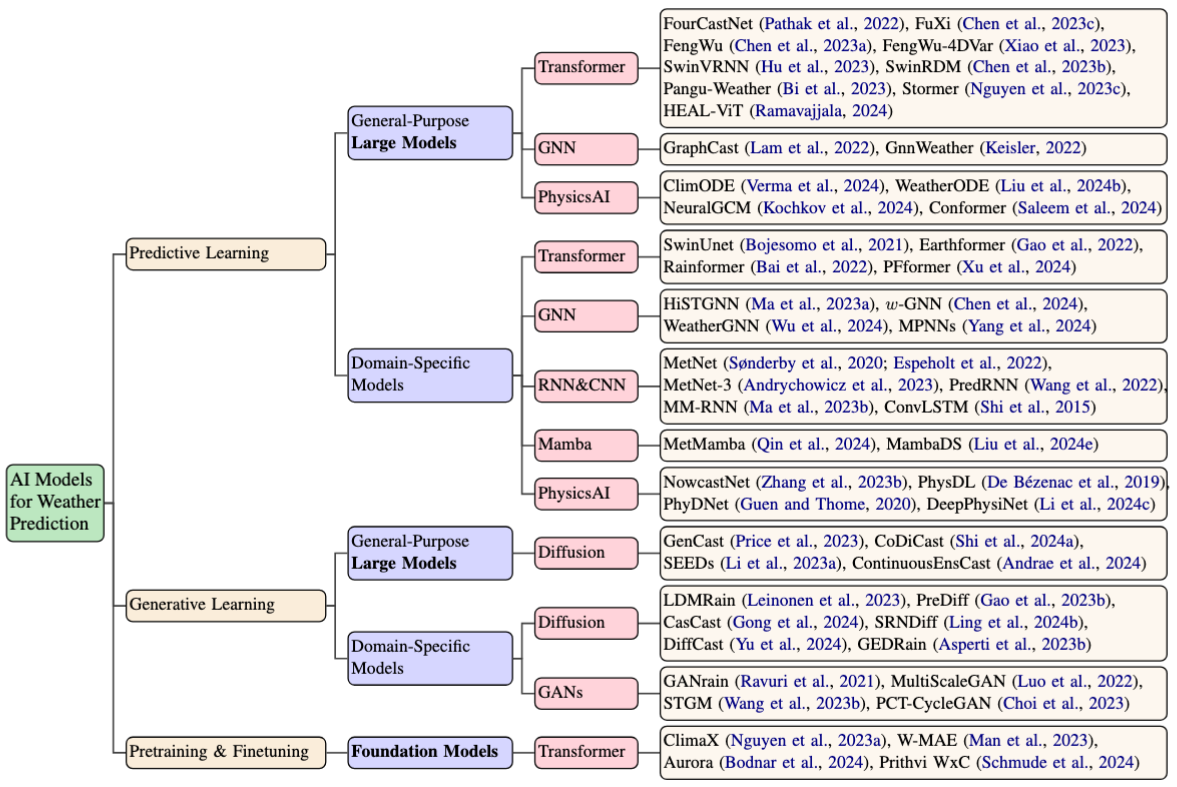
\includegraphics[width=0.8\linewidth]{../figures/review.jpg}
    \caption{Az MLWP-modellek áttekintése. Az ábra Shi et al. (2025) \cite{shi_deep_2025} cikkéből származik.}
    \label{fig:MLWP-review}
\end{figure}

Ahogy az ábrán is látható, az MLWP-modelleknek alapvetően három fajtája van. Legelterjedtebbek az általános célú nagy modellek (\textit{General-Purpose Large Models}), melyek többféle időjárási paraméter globális előrejelzésére alkalmasak. Az operatív időjárás-előrejelzésben kevésbé elterjedtebbek a domén specifikus modellek (\textit{Domain-Specific Models}, melyekkel regionális előrejelzést lehet készíteni egyetlen változóra), illetve az alapmodellek (\textit{Foundation Models}, melyekkel még további finomhangolás, specifikus feladathoz adaptálás lehetséges). Az is megfigyelhető, hogy az utóbbi években a CNN és RNN alapú időjárás-előrejelző modellek háttérbe szorultak a GNN és transzformer architektúrájú modellek mellett. 

A CNN architektúrát LeCun et al. mutatta be 1995-ben \cite{lecun_convolutional_1995}. Az architektúra sturkturált rácsadatok, mint pl. a képek feldolgozására alkalmas; klasszikusan a gépi látás területén (pl. képosztályozás) CNN modelleket használnak \cite{shi_deep_2025}. A CNN-nek négy rétege van (konvolúciós réteg -- \textit{convolutional layer}, gyűjtőréteg -- \textit{pooling layer}, teljesen összekötött réteg -- \textit{fully connected layer} és a nemlineáris réteg -- \textit{nonlinearity layer}), melyeket a \ref{fig:cnn}. ábra szemléltet. A rétegek szerepét egy képosztályozási feladaton keresztül mutatom be.

\begin{figure}[H]
    \centering
    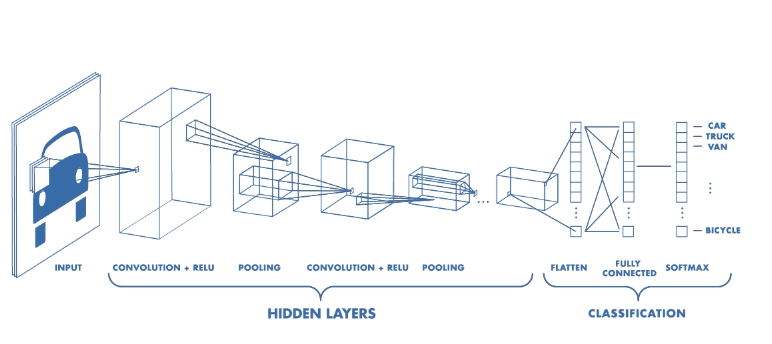
\includegraphics[width=0.8\linewidth]{../figures/cnn.png}
    \caption{A CNN szerkezete. Az ábra Purwono et al. (2022) \cite{purwono_understanding_2022} cikkéből származik.}
    \label{fig:cnn}
\end{figure}

A CNN az inputként kapott képet egy mátrixként látja, ahol a mátrix minden eleme az adott pixel fényintenzitását reprezentálja. A konvolúciós réteg (\textit{convolutional layer}) a képekből a jellemzőket (\textit{feature}, pl. élek, textúrák, minták) nyeri ki. A gyűjtőréteg (\textit{pooling layer}) konvolúciós rétegeket kapcsol össze; szerepe a paraméter- és ezáltal számítási teher csökkentése a konvolúciós réteg kimeneteinek alulmintavételezett reprezentáció készítésével. A teljesen összekapcsolt réteg (\textit{fully connected layer}, más néven konvolúciós output réteg -- \textit{convolutional output layer}) bemenete az utolsó pooling réteg. Az adatot a következő rétegbe továbbítás előtt vektorrá lapítja. Az utolsó réteg a nemlineáris réteg vagy aktivációs függvény (\textit{nonlinearity layer / activation function}); ez a réteg adja meg a neurális hálózat végső kimenetét, a válaszát az adott feladatra \cite{purwono_understanding_2022}.

Az RNN-eket 2001-ben mutatta be Medsker \& Jain \cite{medsker_recurrent_2001}, mint időfüggő vagy szekvenciális adatokkal kapcsolatos feladatok (pl. idősor-előrejelzés) végzésére alkalmas architektúrákat. A modell rekurrens módon tanul a kapott adatsorozatból egy belső rejtett állapot segítségével, ami tartalmazza a korábbi rejtett állapotokat és az aktuális bemenetet. A tanulás folyamatát az alábbi egyenletek írják le:
\[
h_t=\sigma(\mathbf{W}_xx_t+\mathbf{W}_hh_{t-1}+b_h); \quad y_t=\sigma(\mathbf{W}_yh_t+b_y),
\]
ahol a $t$-edik időpillanatban $h_t$ a rejtett állapot, $x_t$ az input, $y_t$ az output; $\mathbf{W}_x, \mathbf{W}_h, \mathbf{W}_y$ súlymátrixok, $b_h, b_y$ bias-ok, $\sigma$ pedig az aktivációs függvény. A CNN-nél és RNN-nél sokkal fontosabb architektúrák azonban az időjárás-előrejelzésben a GNN-ek és a transzformer alapú neurális hálózatok \cite{shi_deep_2025}.

A GNN-t 2008-ban mutatták be Scarselli et al. \cite{scarselli_graph_2008}. Az architektúra $\mathcal{G}=(\mathcal{V, E})$ $\mathcal{V}$ csúccsal és $\mathcal{E}$ éllel rendelkező gráf szerkezetű adatok feldolgozására alkalmas, ahol a csúcsok a vizsgált dolgokat, az élek pedig a köztük fennálló kapcsolatokat reprezentálják. Ha a GNN a tér- és időbeli függőségeket is jól modellezik, tér-idő GNN-ekről (\textit{Spatio-temporal GNN, ST-GNN}) beszélünk, melyeket a $\mathcal{G}_t=\mathcal{(V,E},t)$ jelöléssel szoktak illetni. Itt a csúcsok és az élek térbeli kapcsolatokat írnak le; a vizsgált dolog $i$ térbeli helyen és $t$ időpillanatban felvett vektorát a $v_t^i$ vektor reprezentálja. A térbeli függőségek figyelembevétele az egyes csomópontok szomszédaikkal való kommunikációján (\textit{message passing}) keresztül valósul meg. Az időbeli kapcsolatokat szekvenciális modellekkel (mint az RNN) lehet figyelembe venni. A csomópontok $h_t^i$ rejtett állapotai a $v^i_{t+1}$ üzenetvektorokkal kerülnek frissítésre az alábbi módon:
\[
v_{t+1}^i = \sum_{j \in N(i)} M_t(h_t^i, h_t^j, e_{ij}); \quad h_{t+1}^i = \sigma(h_t^i, v_{t+1}^i),
\]
ahol $N(i)$ az $i$-edik csomópont szomszédjai, $M_t$ az üzenetküldő függvény, $e_{ij}$ pedig az $i$-edik és $j$-edik csomópont közti élet jellemzi \cite{shi_deep_2025}.

Az utóbbi évek legnépszerűbb mesterséges intelligencia-alapú modelljeinek alapjai a transzformer architektúrák. 2017-ben jelent meg Vaswani et al. a transzformer neurális hálózatokat bemutató azóta már nagyon híressé vált cikke, az ,,Attention Is All You Need" \cite{vaswani_attention_2017}. Az architektúra a figyelem mechanizmus (\textit{attention mechanism}) alapján működik; szekvenciális lépések közbeiktatása nélkül képes az adatban fennálló kapcsolatokat megragadni. A figyelem mechanizmus az alábbiak szerint írható le:
\[
\text{Attention}(\mathbf{Q, K, V})=\text{softmax}\left(\frac{\mathbf{QK}^T}{\sqrt{d_k}} \right)\textbf{V},
\]
ahol $d_k$ a \textbf{K} kulcsmátrix (\textit{key matrix}) dimenziója, $\mathbf{Q}\in\mathbb{R}^{n \times d_k}$ a lekérdezési mátrix (\textit{query matrix}), $\mathbf{K}\in\mathbb{R}^{m \times d_k}$ a kulcsmátrix, $\mathbf{V}\in\mathbb{R}^{m \times d_v}$ az értékmátrix (\textit{value matrix}). Ezeket a mátrixokat az $\mathbf{X}\in \mathbb{R}^{n \times d}$ bemeneti szekvenciális adatokat tartalmazó mátrix alapján az alábbiak szerint számolják ki:
\[
\mathbf{Q=XW_q, \quad K=XW_k, \quad V=XW_v},
\]
ahol $\mathbf{W_q} \in \mathbb{R}^{d \times d_k}, \mathbf{W_k} \in \mathbb{R}^{d \times d_k}, \mathbf{W_v} \in \mathbb{R}^{d \times d_v}$ rendre a \textbf{Q, K, V} mátrixokhoz tartozó tanulható súlymátrixok \cite{shi_deep_2025}.

A Vision Transformer-t (\textit{ViT}) Dosovitskiy et al. mutatta be 2021-ben \cite{dosovitskiy_image_2021}. Ez egy olyan transzformer, amely képek feldolgozására lett kifejlesztve. A ViT a bemenetként kapott képet rácsos szerkezetben részekre (\textit{patch}) osztja; ezeket az adat-darabokat (úgynevezett \textit{tokeneket}) alakítja aztán vektorrá és dolgozza fel. Az így előkészített tokeneket továbbítják aztán egy transzformerbe, ahol a figyelem mechanizmus már alkalmazható. A Vision Transformer szerkezetét mutatja a \ref{fig:vit}. ábra.

\begin{figure}[H]
    \centering
    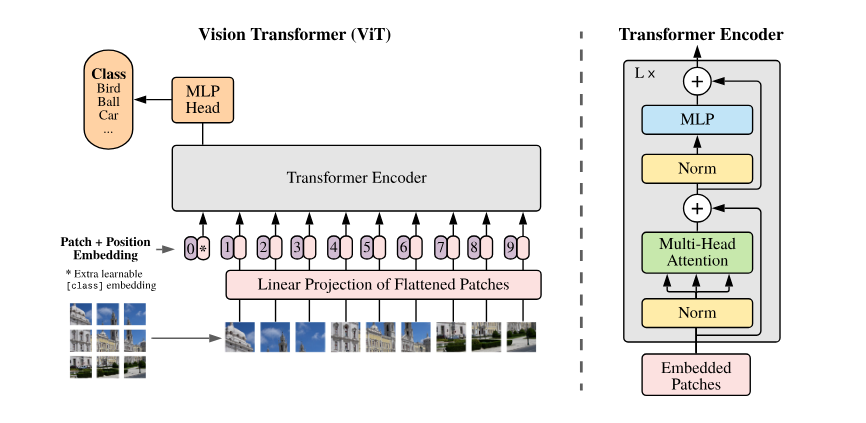
\includegraphics[width=0.8\linewidth]{../figures/vit.png}
    \caption{A ViT szerkezete. Az ábra Dosovitskiy et al. (2021) \cite{dosovitskiy_image_2021} cikkéből származik.}
    \label{fig:vit}
\end{figure}

\subsection{Kaotikus neurális hálózatok}

A káosz görög eredetű szó, eredeti jelentése ,,tátongó űr". Máshogy megfogalmazva a káosz egy komplex rendszer viselkedésében megnyilvánuló teljes zűrzavar vagy kiszámíthatatlanság. A káoszt a kezdeti feltételekre való rendkívüli érzékenységgel szokás azonosítani, ami a hosszútávú idősor-előrejelzést lehetetleníti el. Ezt először Henri Poincaré francia matematikus figyelte meg a 19. században, majd 1963-ban Edward Lorenz angol matematikus és meteorológus fogalmazta meg a káoszelméletet; tőle származik a ,,pillangóhatás" kifejezés is. Lorenz egy modellt készített, ami a légköri mozgásokat hivatott reprezentálni. A számításai során látszólag elhanyagolható kerekítéseket végzett, azonban észrevette, hogy ez az előrejelzésben rendkívül nagy eltéréseket okozott. Ez a kezdeti feltételekre való érzékenység koncepciója. Az 1989-ben Benoît Mandlebrot fedezte fel a fraktálok (önhasonló objektumok; a ,,káosz mintázatai") jelentőségét a kaotikus attraktorok leírásában. \cite{biswas_chaos_2018, anusree_understanding_2025}. 

Ahhoz, hogy egy rendszer kaotikusnak nevezhessünk, az alábbi jellemzőknek kell teljesülnie:
\begin{itemize}
    \item Nem jelenik meg periodikusság.
    \item Kezdeti feltételekre való érzékenység.
    \item Kaotikus mozgást nehéz vagy lehetetlen előrejelezni.
    \item Véletlenszerűnek látszó (de valójában determinisztikus) mozgás.
    \item Nemlineáris.
\end{itemize}

A kaotikus neurális hálózatokat (\textit{Chaotic Neural Network, cNN}) -- a káoszelmélet és neurális hálózatok ötvözetét -- Aihara et al. mutatták be 1990-ben \cite{aihara_chaotic_1990}.  A cNN-ek a kaotikus rendszerek komplex mintázatait képesek reprezentálni és változatos megoldásokat tudnak felfedezni. A cNN neuronjai nemlineáris aktivációs függvények által kaotikus dinamikát mutatnak, amely egy ún. bifurkációs paraméter változtatásával szabályozható. Ez azért hasznos, mert így a neurális hálózat komplex -- kaotikus -- kapcsolatokat is felfedezhet az adatok közt. \cite{anusree_understanding_2025}. A kaotikus neuron szerkezetét a \ref{fig:chaotic_neuron}. ábra mutatja be.

\begin{figure}[H]
    \centering
    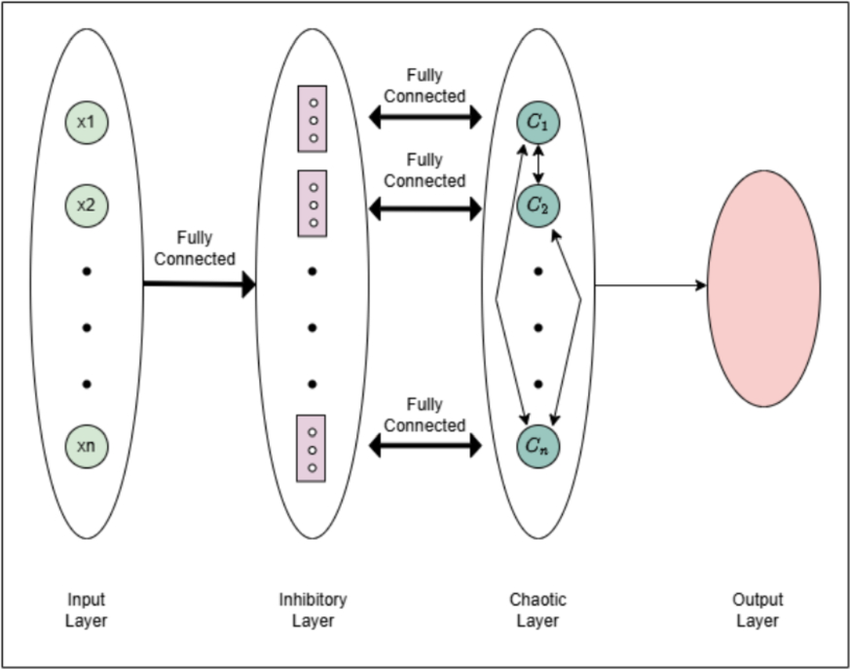
\includegraphics[width=0.5\linewidth]{../figures/chaotic_neuron.png}
    \caption{A kaotikus neuron szerkezete Crook \& Scheper (2001) \cite{crook_novel_2001} alapján. Az ábra Anusree \& Pramod (2025) \cite{anusree_understanding_2025} cikkéből származik.}
    \label{fig:chaotic_neuron}
\end{figure}

A bemutatott kaotikus neuron három rétegből áll. A bemeneti (\textit{input}) réteg fogadja a bejövő dinamikus jeleket. A réteg teljesen össze van kötve (\textit{fully connected}) egy gátló neuronokból álló klaszterek alkotta réteggel (\textit{inhibitory layer}). Egy-egy ilyen klasztert alkotó neuronok mindegyik a következő, kaotikus (\textit{chaotic}) réteg ugyanazon neuronjához kapcsolódik. A kaotikus réteget alkotó minden egység teljes összeköttetésben van a többi egységgel \cite{anusree_understanding_2025}. 

A cNN-ek tehát le tudják képezni a kaotikus jellemzőket. Jelenleg azonban főként arra használják a technológiát, hogy a tanítás során a modell ne ragadjon bele lokális minimumokba  \cite{anusree_understanding_2025}. Az Echo State Network-öt (\textit{ESN}) -- egy olyan neurális hálózat, ami bizonyos körülmények között képes kaotikus tulajdonságokat produkálni -- Ortiz et al. (2025) \cite{ortiz_exploring_2025} már használták a meteorológia területén, felhőzet-előrejelzésre. Azonban a kaotikus neurális hálózatok gépi tanulás alapú időjárás-előrejelző modellekbe való integrálása még nem terjedt el széleskörűen, nem találkoztam ilyen jellegű tanulmányokkal a szakirodalmi kutatásom során.


\subsection{Gépi tanulás alapú időjárás-előrejelző modellek}

Az időjárás-előrejelzés területén a gépi tanulást már több, mint 25 éve használják (ld. pl. Hung et al., 2009, akik ANN-t használtak az eső előrejelzésére Bangkokban \cite{hung_artificial_2009}), azonban csak az utóbbi években ért el a technológia olyan fejlettséget, hogy operatív, több időjárási változóra is kiterjedő előrejelzést lehessen készíteni segítségével \cite{de_burgh-day_machine_2023}. 

Az első jelentősebb ANN architektúrán alapuló MLWP-modell az NVIDIA 2022-ben bemutatott, Fourier neurális hálózat alapú FourCastNet (\textit{FOURier ForeCASTing Neural NETwork}) nevű modellje. Az architektúra alapötlete a fentebb már ismertetett ViT. Azonban a ViT erőforrásigénye a pixelszámokkal négyzetesen nő, így sokdimenziós bemeneti adatoknál már nem érdemes használni. Ezen probléma áthidalására fejlesztették ki Guibas et al. 2022-ben az Adaptív Fourier Neurális Operátorokat (\textit{Adaptive Fourier Neural Operator, AFNO}). A módszer a függvények Fourier-terén hat, ami sok számítást leegyszerűsít (pl. a konvolúcióból szorzás lesz). Az AFNO lényegében a ViT módszert váltja fel \cite{pathak_fourcastnet_2022, guibas_adaptive_2022}.

Szintén híres MLWP-modell a Huawei által 2023-ban bemutatott Pangu-Weather. A modell egy ún. 3D-s Föld-specifikus transzformer (\textit{3D Earth-Specific Transformer, 3DEST}), melynek szerkezetét a \ref{fig:3DEST}. ábra mutatja be.

\begin{figure}[H]
    \centering
    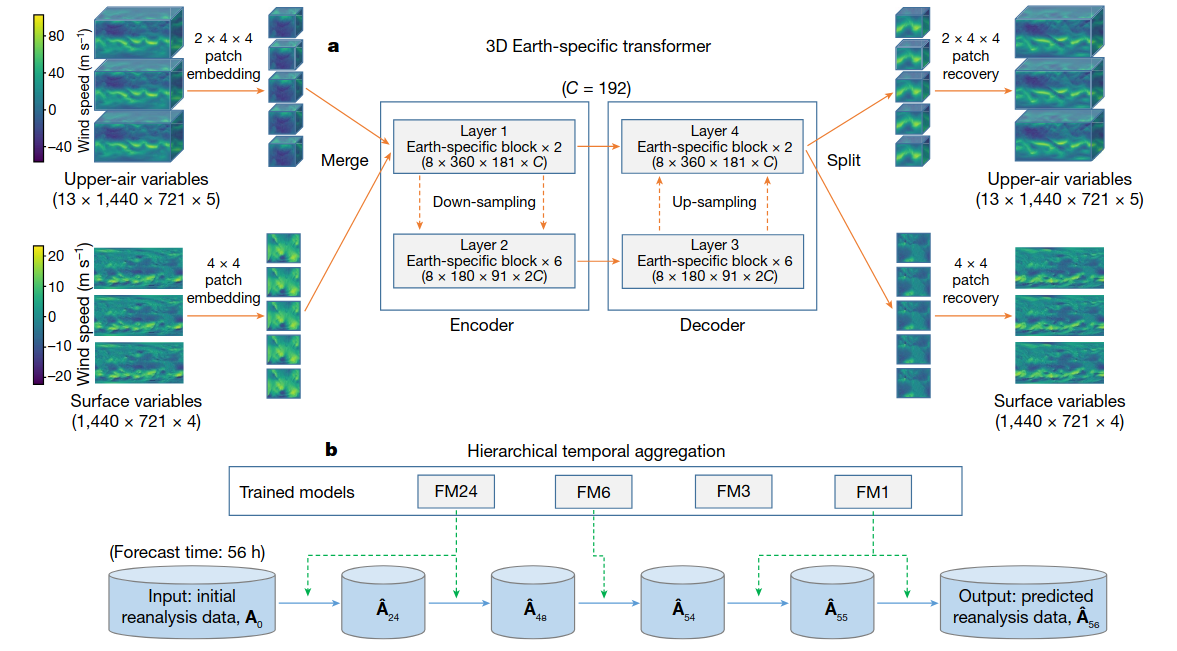
\includegraphics[width=0.8\linewidth]{../figures/3DEST.png}
    \caption{A 3DEST szerkezete. Az ábra Bi et al. (2023) \cite{bi_accurate_2023} cikkéből származik.}
    \label{fig:3DEST}
\end{figure}

A 3DEST architektúra a bemenő adatokon ún. \textit{patch embedding}et végez, ami során a térbeli felbontást lecsökkenti és egy 3D-s kockába sűríti. Ezt követően a hálózat a 3D-s adatokat egy enkóder-dekóder architektúrába továbbítja, ami jelen esetben egy Swin-transzformer, ami a ViT egy fajtája. Az enkóder-dekóder architektúra által átalakított adatokon ezt követően \textit{patch recovery}t hajt végre, hogy az eredeti felbontást visszakapjuk. A modell célja középtávú (7+ nap) előrejelzések készítése volt, ami eléréséhez egy ún. \textit{hierarchical temporal aggregation} módszert, egy ,,mohó algoritmust" (\textit{greedy algorithm}) alkalmaztak. Mivel a neurális hálózatok rövid időtávra (1, 3, 6, 24 óra) pontosabban tudnak előrejelezni, a hosszabb távú előrejelzéseket rövidebb távúakból hierarchikusan állítják elő. Például ha 56 órára készítenek előrejelzést, először két 24 órás előrejelzést készítenek. A fennmaradó $56-2\cdot24=8$ órát egy 6 órás és 2 db 1 órás előrejelzéssel fedik le. Ezáltal az előrejelzési hibák kevésbé halmozódnak fel, mintha pl. 56 db 1 órás előrejelzést raknának össze \cite{bi_accurate_2023}.

A következő bemutatott modell a Google által szintén 2023-ban publikált, GNN-alapú GraphCast modellje. A GNN-ek működése fentebb már említésre került. A modell a számításokat egy ún. \textit{multi-mesh}-en -- magas felbontású, ikozaéderes gráfon -- végzi. A modellben enkóder-processzor-dekóder architektúra található. Az 1 GNN-rétegből álló enkóder 6-szoros iteratív finomítás után az ikozaéder csomópontjait (\textit{node}-jait) a földgömbre vetíti; ezzel létrejönnek $M^0 ... M^6$ rácshálózat, ahol $M^0$ a legdurvább, $M^6$ pedig a legfinomabb felbontást jelenti. A teljes \textit{multi-mesh} mind a 7 rácshálózatot magában foglalja. A 16 GNN-réteget magában foglaló processzor a \textit{multi-mesh}-en az információ továbbítását tanulja. A szintén 1 GNN-rétegből álló dekóder a \textit{multi-mesh}-en megtanult jellemzőket visszavetíti a földrajzi fokhálózatra. A \textit{multi-mesh} egyik előnye, hogy -- szemben a hagyományos földrajzi fokhálózattal -- térben homogén, nincsen pl. a pólusokon \textit{node} felgyülemlés. A másik legnagyobb előnye, hogy a többféle felbontású rácshálózatokat magában foglaló \textit{multi-mesh}-en hatékonyabb az információ továbbítása: egy távoli pontba pl. először a legdurvább $M^0$-n, majd egyre finomabb rácshálókon halad az információ. A GraphCast modell működését a \ref{fig:graphcast}. ábra szemlélteti \cite{lam_graphcast_2023}.

\begin{figure}[H]
    \centering
    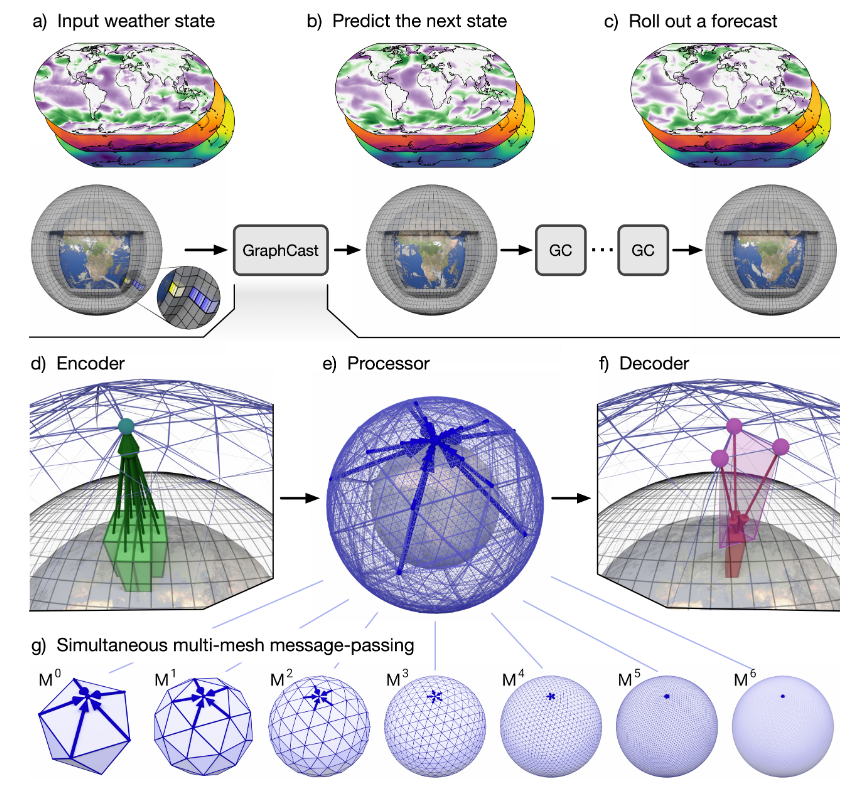
\includegraphics[width=0.8\linewidth]{../figures/graphcast.png}
    \caption{A GraphCast modell működése. Az ábra Lam et al. (2023) \cite{lam_graphcast_2023} cikkéből származik.}
    \label{fig:graphcast}
\end{figure}

A Chen et al. által 2023-ban bemutatott FuXi MLWP-modell három részből áll: a kocka beágyazásból (\textit{cube embedding}), egy U-transzformerből, illetve egy egy teljesen összekötött (\textit{fully connected}) rétegből. A \textit{cube embedding} célja a bemenő sokdimenziós adat idő- és térbeli dimenzióinak, ezáltal redundanciájának csökkentése. Az adatok feldolgozását egy U-transzformer végzi. Az adatdimenzió csökkentését egy alulmintavételező egység, a \textit{Down Block} végzi. Ezt követően 48 egymás utáni Swin-transzformer típusú ViT-ből dolgozza fel az adatokat. Végül az adatok dimenziójának növelését egy felülmintavételező egység, az \textit{Up Block} végzi. A modell felépítését a \ref{fig:fuxi}. ábra mutaja be \cite{chen_fuxi_2023}.

\begin{figure}[H]
    \centering
    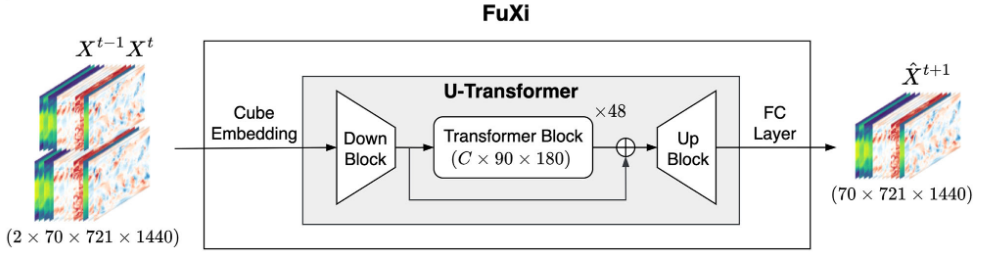
\includegraphics[width=0.8\linewidth]{../figures/fuxi.png}
    \caption{A FuXi modell áttekintő szerkezete. Az ábra Chen et al. (2023) \cite{chen_fuxi_2023} cikkéből származik.}
    \label{fig:fuxi}
\end{figure}

Az ECMWF által 2024-ben bemutatott Artificial Intelligence Forecasting System (AIFS) modell több korábban bemutatott MLWP-modell előnyeit ötvözi; egyszerre GNN és transzformer alapú is. Az ERA5 rácshálózatról a processzor alacsonyabb felbontású oktaéderes gráfhálózatára vetítő enkóder és a visszalakítást végző dekóder GNN-transzformer (\textit{,,GNN attention"}) architektúrával rendelkezik. A processzor tisztán transzformer alapú, 16 db Swin-transzformer rétegből áll. A processzor a rácshálózatot alkotó gráf minden pontjának környezetét is figyelembe veszi egy adott levágási (\textit{cut-off}) sugáron belül.

\subsection{MLWP-modellek kaotikus tulajdonságai}

Azt, hogy megállapítsuk, hogy egy modell tudja-e a kaotikus jegyeket produkálni, legegyszerűbben az előrejelzésben valamilyen kezdeti perturbáció növekedésének vizsgálatával tehetjük meg. Ha a hiba exponenciálisan nő (azaz találunk pozitív Ljapunov-exponenst), a káosz jelen van a predikcióban.

Ezt vizsgálták 2023-ban Selz \& Craig kis perturbációval ellátott ensemble (együttes) előrejelzések segítségével. A vizsgált modellek az MLWP-típusú Pangu-Weather és az NWP-típusú ICON modellek voltak; a modell-előrejelzések perturbációra adott válaszát vizsgálták. Azért fontos, hogy a perturbáció kicsi legyen, mert a nagy perturbáció elnyomja a modell-specifikus effektusokat, és az MLWP-modell úgy viselkedik, mint a hagyományos NWP-modellek. Az NWP-modellek alapján várható lenne, hogy a légkör kaotikussága miatt a hozzáadott kis hiba exponenciálisan kezd el nőni, ami az időjárás-előrejelzésnek egy inherens időbeli felső korlátot ad (,,pillangó-hatás"). Ezzel szemben Selz \& Craig azt tapasztalták, hogy a Pangu-Weather nem képes reprodukálni ezt a kezdeti exponenciális hibanövekedést, amivel egy hamis biztonságérzetet ad a hosszútávú időjárás-előrejelzések megbízhatóságára \cite{selz_can_2023}.

Vizsgálatuk során kis- és nagy felbontású rácshálózatot is alkalmaztak. A nagy felbontású rácson (2,5 km) a konvekció -- a légkör egyik legkevésbé lineáris folyamata -- is megfigyelhető legyen. A vizsgálat esettanulmány-jellegű, 2021. június 26. 00 UTC inicializációs idejű előrejelzéseket használtak fel. Az időpont-választás oka, hogy ekkor Észak-Amerika felett -- nyár lévén -- nagyon jelentős konvekciós folyamatok zajlottak; azonban eredményeiket az egész Földre átlagolva adták meg \cite{selz_can_2023}.

A hibanövekedés számszerűsítésére egy ilyen célra gyakran használt mennyiséget, a 300 hPa-on számolt kinetikus energia-különbséget (\textit{Difference Kinetic Energy, DKE}) alkalmazták:
\[
\text{DKE}=\text{Var}(u) + \text{Var}(v),
\]
ahol $u$ és $v$ a horizontális szélkomponensek \cite{selz_can_2023}. 

A kutatók kis- és nagyobb perturbációkat is végeztek; eredményeiket a \ref{fig:selz-pert}. ábra foglalja össze.

\begin{figure}[H]
    \centering
    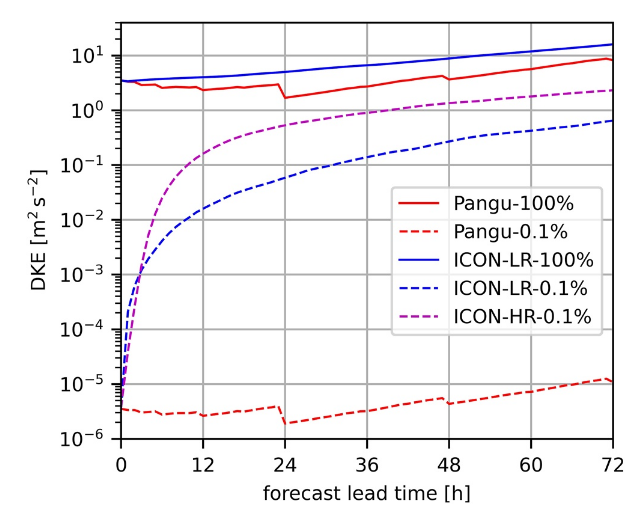
\includegraphics[width=0.5\linewidth]{../figures/selz-pert.png}
    \caption{Az ICON és Pangu-Weather (\textit{Pangu}) nagy (\textit{100\%}) és kicsi (\textit{0.1 \%}) perturbációkra adott válaszai a DKE növekedésén keresztül bemutatva. A \textit{HR} a nagy felbontást (2.5 km), a \textit{LR} az alacsony felbontást (20 km) jelent. Az ábra Selz \& Craig (2023) \cite{selz_can_2023} cikkéből származik.}
    \label{fig:selz-pert}
\end{figure}

A nagy perturbáció során alátámasztásra került a várakozásuk, hogy az elnyomja az MLWP-modell jellegzetességeit: az erősen perturbált Pangu-Weather (\textit{Pangu-100\%}) hasonlóan viselkedett, mint az erősen perturbált ICON (\textit{ICON-LR-100\%}). A kicsit perturbált ICON (\textit{ICON-0.1\%}) esetében is az NWP-modellektől elvárható eredményre jutottak: a hiba nagyon gyorsan kezdett nőni, míg szaturációba nem került (48 óra után a hibanövekedési ütem kb. megegyezett az erősen perturbált ICON-éval). Ha az alacsonyabb felbontású, kicsit perturbált modellt (\textit{ICON-LR-0.1\%}) a magasabb felbontásúhoz (\textit{ICON-HR-0.1\%}) hasonlítjuk, megfigyelhető, hogy az alacsonyabb felbontású alulbecsli a hibát már néhány óra elteltével. Ennek oka az lehet, hogy a kis felbontás miatt nincsenek megfelelően reprezentálva a hibához jelentősen hozzájáruló nemlineáris konvektív folyamatok \cite{selz_can_2023}.

A kicsit perturbált Pangu-Weather modell hibanövekedésének időbeli lefutása nagyon hasonló az erősebben perturbáltéhoz; az eltolás a hibában a perturbáció mértékével arányos. A Pangu-Weather az ICON modellhez képest alulbecsli a hibát és konstans hibanövekedést mutat az exponenciális helyett, ami -- helytelenül -- sokkal hosszabb távú előrejelezhetőséget sugall \cite{selz_can_2023}.

Azonban a fent említett vizsgálat elvégzéséhez -- tekintve, hogy az ensemble előrejelzések sok tagból állnak -- rendkívül magas számítási kapacitásra van szükség. Selz \& Craig pl. az ECMWF Atos nevű szuperszámítógépét használták. A Pangu-Weather kísérletek 16, az alacsony felbontású ICON-kísérletek 2900, a magas felbontású ICON-kísérletek pedig 1300000 számítási órába kerültek egyenként \cite{selz_can_2023}.

Ennél olcsóbb módszerek lehetnek az előrejelzési idősorban való kaotikus viselkedés észlelése, vagy trajektóriamodellezés.

Az előrejelzési idősorban való kaotikus viselkedés észlelésére felhasználható módszerekkel foglalkozik Pánis et al. 2020-as cikke \cite{panis_detection_2020}.

A kaotikus rendszereket fázistérben (pl. sebesség-kitérés koordináta-rendszer) ábrázolva komplex, de rendezett, fraktálszerű alakzatot kapunk. A fraktálok olyan geometriai alakzatok, melyek kerülete és felülete nincs definiálva és önhasonlóak; ezt szemlélteti a \ref{fig:koch}. ábrán feltüntetett híres példa, a Koch-görbe, melynek területe véges marad ugyan, de kerülete a végtelenhez tart \cite{tel_kaotikus_2002}.

\begin{figure}[H]
    \centering
    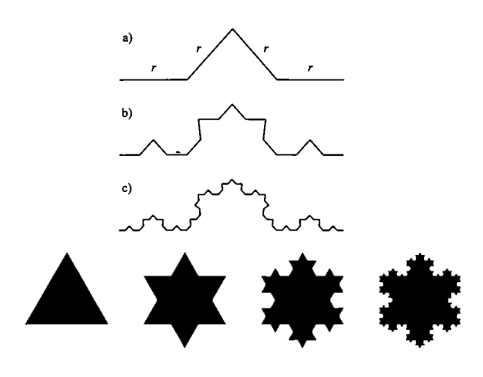
\includegraphics[width=0.5\linewidth]{../figures/koch.png}
    \caption{A Koch-görbe szerkesztése és fraktálszerkezete. Az ábrák Tél \& Gruiz Kaotikus dinamika című tankönyvéből (2002) származnak \cite{tel_kaotikus_2002}.}
    \label{fig:koch}
\end{figure}

A fraktálokat fraktáldimenzióval szokás jellemezni, ami síkbeli (térbeli) alakzatoknál egynél (kettőnél) nagyobb, de kettőnél (háromnál) kisebb tört vagy irracionális szám; a dimenzió nagysága az alakzat tagoltságával arányos. Fedjük le ezeket az alakzatokat $\varepsilon$ karakterisztikus méretű dobozokkal (\textit{box}-okkal). Míg pl. egy hagyományos síkbeli alakzat lefedéséhez $\varepsilon^{-2}$-el arányos az alakzat egyre finomabb lefedéséhez szükséges dobozok száma, addig fraktáloknál a kitevő egy nem egész szám, a fraktáldimenzió lesz:
\[
N(\varepsilon)\propto \varepsilon^{-D_0},
\]
ahol $\varepsilon \rightarrow 0$, $N$ az alakzat lefedéséhez szükséges minimális számú doboz, $D_0$ pedig a fraktáldimenzió. Átrendezve:
\[
D_0=\lim_{\varepsilon \rightarrow 0}\frac{\ln N(\varepsilon)}{\ln 1/\varepsilon}
\]
adja meg a fraktáldimenziót. A box-counting módszer arra épül, hogyha tudunk ilyen fraktáldimenziót találni, akkor a vizsgált idősor kaotikus jeleket mutat \cite{tel_kaotikus_2002,panis_detection_2020}.

Másik módszer az idősor-adatokban a káosz észlelésére a korrelációs dimenzió ($D_2$) vizsgálata. A korrelációs dimenzió kiszámítása során megszámoljuk, hogy hány pontpár ($C(\varepsilon)$) van egymáshoz közelebb, mint egy nagyon kicsi $\varepsilon$ küszöbérték:
\[
D_2=\lim_{\varepsilon \rightarrow 0}\frac{\ln C(\varepsilon)}{\ln \varepsilon}.
\]
Ha találunk korrelációs dimenziót, az idősor kaotikus \cite{panis_detection_2020}.

Következő módszer a Ljapunov-exponens keresése. Ha a kaotikus attraktor egy $\mathbf{r}$ pontja körül két közeli pontból indítunk részecskéket, távolságuk a lépések $n$ számának növelésével exponenciálisan nőni fog:
\[
\Delta r_n=\Delta r_0 e^{\bar{\lambda}n},
\]
ahol $\Delta r_0$ a kezdeti (kicsi) távolságuk, $\bar{\lambda}$ pedig a fázistérhez rendelhető átlagos Ljapunov-exponens. Kaotikus rendszerekben $\bar{\lambda}>0$. Ha az idősorban sikerül pozitív Ljapunov-exponenst találni -- pl. egyenesillesztéssel --, akkor a rendszer, ahonnan az idősor származik, kaotikus \cite{panis_detection_2020}.

A gépi tanulást a kaotikus viselkedés detektálására is használhatjuk. Alkotható olyan modell, amely a kaotikus minták felismerésére van tanítva, így az ember számára nehezen felismerhető vagy észrevétlenül maradt mintázatokat is képes felismerni \cite{panis_detection_2020}.

A kaotikus jelek detektálására használhatóak lagrange-i trajektória modellek is: szimulálható segítségükkel, hogy a légkör egy térfogatdarabja (pl. egy szennyezés) hogyan változtatja térfogatát, növeli időben exponenciálisan a szálainak a hosszát, majd áll rá a kaotikus attraktorra \cite{haszpra_replat_2014}.

A terjedési modellek célja, hogy a meteorológiai viszonyok (szélvektor) ismeretében modellezzék, hogy a légkörben egy részecske hogyan terjed. A terjedési modellek időjárás-előrejelző modellekkel vannak meghajtva, azok szélviszony-előrejelzései szolgáltatják a széladatokat a részecske mozgásának modellezéséhez. A terjedési modellekkel figyelembe lehet venni a felszínközeli viszonyokat, mint a súrlódás, azonban az bonyolulttá teszi a modellt. Ha alacsonyabb nyomású izobárszinteken vizsgáljuk a részecskék terjedését, dominánsan csak a szél fogja befolyásolni a részecske terjedését, így a súrlódás elhanyagolhatóvá válik. 

A szimulált trajektóriák felhasználásával is ki lehet mutatni a káosz jelenlétét, legegyszerűbben a topologikus entrópia ($h$) segítségével tehető ez meg. A mennyiség jellemzi egy kezdetben $L_0$ hosszú fonaldarab megnyúlását:
\[
L(t)=L_0 \cdot e^{ht} \quad (t\gg 1/h),
\]
tehát a mozgás bonyolultságával van kapcsolatban: minél nagyobb $h$, annál bonyolultabb lesz a mozgás (jobban megnyúlik a kezdeti fonaldarab). Ha $h>0$, a mozgás kaotikus. A topologikus entrópia becslése sok részecske pályájának nyomon követésével lehetséges \cite{haszpra_ensemble-based_2019}.


\section{Adat, módszer}
Vizsgálataim során 2 dimenziós trajektóriamodellt hajtottam meg 2026. június 1-én UTC szerint 0 órakor készült ECMWF-IFS, illetve ECMWF-AIFS szél-előrejelzésekkel. Az előrejelzések középtávúak (360 órára előre készülnek el 6 órás lépésekkel), determinisztikusak, és jelentős számú izobárszintre (1000, 925, 850, 700, 600, 500, 400, 300, 250, 200, 150, 100, 50 hPa) elkészülnek $0,25^\circ \times 0,25^\circ$ globális térbeli felbontással.

\subsection{A trajektóriamodell}
Trajektóriamodellnek egy, a témavezetőm által biztosított, Python nyelven írt modellt vettem alapul. Ezt jelentősen átalakítva, illetve további funkciókkal bővítve használtam fel.

A modell bemenetként várja:
\begin{itemize}
    \item Szélességi kör intervallum mintavételezési sűrűséggel, ahonnan a részecskéket indítjuk (\textit{ndarray adattípus, tetszőleges dimenzió}).
    \item Hosszúsági kör intervallum  mintavételezési sűrűséggel, ahonnan a részecskéket indítjuk (\textit{ndarray adattípus, szélességi körök array-ével megegyező dimenzió}).
    \item Eredeti ECMWF előrejelzések indítási ideje (\textit{yyyymmdd formátumban, int adattípus}).
    \item Előrejelzési időtartam (\textit{értéke legfeljebb 360, int adattípus}).
    \item Vizsgált izobárszint (\textit{értéke az ECMWF által használt főizobárszintek valamelyike lehet, int adattípus}).
\end{itemize}

Mivel a modellelőrejelzések csak 6 óránként állnak rendelkezésre, a trajektóriamodell lineáris interpolációt végez a köztes időpillanatok szélsebességének kiszámítására, amivel egy időben folytonosan változó szélsebesség-mezőt hoz létre.

Az elengedett részecskék trajektóriájának kiszámításához a következő differenciálegyenlet-rendszert szükséges megoldani minden részecskére:
\begin{equation}\label{eq:lambda}
\frac{d \lambda}{d t} = u\cdot C \cdot \frac{1}{\cos \varphi},
\end{equation}
\begin{equation}\label{eq:phi}
\frac{d \varphi}{d t} = v \cdot C,
\end{equation}
ahol $u$ a keleti (zonális)-, $v$ pedig az északi (meridionális) szélkomponens m/s-ban; $C$ egy váltószám, ami a m-t $^\circ$-ba váltja át ($C=\frac{180 ^\circ}{\pi \cdot R}$, ahol $R=6371000$ m a Föld sugara); $\lambda$ a részecske (keleti) hosszúsági koordinátája, $\varphi$ az (északi) szélességi koordinátája; $t$ pedig a szimulációs idő másodpercben. A 0-val való osztást úgy akadályozzuk meg, hogy a szélességi köröket csak $-89,9^\circ$ és $89,9^\circ$ között vesszük. A differenciálegyenlet-rendszert az elterjedt Runge-Kutta 5(4) rendű módszer segítségével integráltam numerikusan. A Runge-Kutta módszer adaptív időlépésekkel dolgozik. Az esetlegesen fellépő túl nagy időlépés alkalmazását úgy akadályoztam meg, hogy a maximális lépésközt 10 percre állítottam. A relatív és abszolút hibatoleranciát is $10^{-3}$-nak vettem.

A szimulációkkal fő célom topologikus entrópia meghatározása volt, amihez a részecskék által kifeszített fonal hosszának időbeli változását szükséges vizsgálni. Azonban ha túl messzire kerül egymástól két szomszédos részecske, a köztük lévő, koordinátáik felhasználásával egyszerűen számítható, légvonalbeli távolság nem fog megegyezni a köztük lévő fonaldarab hosszával. Ennek kiküszöbölésére ha két szomszédos részecske egymástól több, mint 20 km távolságra került, beszúrtam egy részecskét közéjük. A dinamikus részecskebeszúrással előállított trajektóriákat kezdetiérték-vektor felülírással ciklusban léptetett Runge-Kutta módszerrel integráltam.

Az ilyen módon előállított, megfelelően sűrű részecskehálózatban jó közelítés a szomszédos részecskék közti fonaldarab hosszára a légvonalbeli $d$ távolságuk, melyet a Haversine-formulával számítottam:
\[
d=R \cdot 2 \cdot \arcsin \sqrt{\sin\left(\frac{\Delta \varphi}{2} \right)^2 + \cos \left(\varphi_1 \right)\cdot\cos(\varphi_2)\cdot\sin\left(\frac{\Delta \lambda}{2} \right)^2},
\]
ahol $(\varphi_1, \lambda_1)$ és $(\varphi_2, \lambda_2)$ a két részecske koordinátája, $\Delta \varphi$ szélességi radián különbségük, $\Delta \lambda$ hosszúsági radián különbségük, $R=6371000$ m pedig a Föld sugara.

A trajektóriamodell futtatása 8 magos AMD Ryzen 7 2700X processzor alapú számítógépen történt. A részecskebeszúrást végző metódussal ellátott modell jelentősen megnövekedett lineáris algebrai számítási terhelést jelentett a részecskék megugró száma miatt. A futási időt a NumPy által támogatott többszálú végrehajtás engedélyezésével csökkentettem.

\subsection{Felhasznált adat}

A modellt ECMWF-IFS, illetve ECMWF-AIFS szélelőrejelzésekkel is meghajtottam.A vizsgálatokat több izobárszinten (850, 700, 500 hPa) végeztem, 168 órás előrejelzési időtávra. Az előrejelzési időtáv megválasztása azért történt így, mert ez már elég hosszú idő ahhoz, hogy reprezentatív lenyomatot kaphassunk a légkör folyamatairól. Emellett elég rövid ahhoz, hogy a szimulációknak -- a jelentősen megnövekvő részecskeszám miatt -- ne teljen túl sok időbe lefutniuk. 

A felhasznált ECMWF-előrejelzések az ECMWF-modellek legújabb verzióival készültek: a 2026. május 12-én megjelent IFS Cycle 50r1-gyel, illetve AIFS v2-vel \cite{snell_significant_2026}. A felhasznált előrejelzések futtatási idejei: 2026. június 1., 2026. július 1., 2026. augusztus 1., 2026. szeptember 1., 2026. október 1.

A részecskéket tetszőlegesen kiválasztott tértartományból lehet indítani. A vizsgálatom során egy adott hosszúsági kör mentén 10$^\circ$-nyi szélességi kört vettem figyelembe több helyen:
\begin{itemize}
    \item K.h. 20$^\circ$ mentén é.sz. $[45^\circ, 55^\circ]$, mivel ez Magyarország területét is magában foglalja.
    \item K.h. 20$^\circ$ mentén é.sz. $[50^\circ, 60^\circ]$, az északi poláris jet stream helyszíne.
    \item K.h. 20$^\circ$ mentén é.sz. $[10^\circ, 20^\circ]$, a passzát szél helyszíne.
\end{itemize}


A k.h. 20$^\circ$, é.sz. $[45^\circ, 55^\circ]$, illetve a jet stream tértartományára a 2026. szeptember 1-i adatokkal nem sikerült lefuttatnom a modellt, melynek okait a Diszkusszió fejezetben fogom tárgyalni.

\subsection{Kaotikus viselkedés számszerűsítése}
A modellezett trajektóriák felhasználásával topologikus entrópiát számoltam. Ehhez a szimuláció minden időlépésében szükséges kiszámolni a részecskéket képzeletben összekötő, egyre bonyolultabb alakot felvevő fonal hosszát. Ez úgy tehető meg, hogy az adott időlépésben a részecskék koordinátáinak ismeretében kiszámolom, milyen messze vannak egymástól a szomszédos részecskék, és ezeket a távolságokat összeadom. Ha a részecskék elég sűrűen helyezkednek el, ezzel a módszerrel viszonylag pontosan megkapható a fonal megnyúlásának időfüggése, a kapott adatokra való illesztéssel pedig egyszerűen meghatározható a $h$ topologikus entrópia. Az elég sűrű elhelyezkedést 20 km-es távolságküszöbbel dinamikus részecskebeszúrással biztosítottam.

A rendelkezésre álló adatok $0,25^\circ \times 0,25^\circ$ felbontásúak, ami kb. 27 km $\times$ 27 km-es felbontást jelent. Ez trajektóriák modellezésekor meglehetősen durva felbontásnak számít, a szakirodalomban ennél jóval finomabb felbontást -- pl. 300-600 m -- használnak \cite{haszpra_ensemble-based_2019}. A részecskéket egymástól $0,005 ^\circ$-ra indítottam, ami kb. 540 m-t jelent. Tizedekkora felbontáson ($0,05^\circ \times 0,05^\circ$) nem volt jelentős szimulációs idő csökkenés, így maradtam a finomabb felbontásnál. A modell minden lépésben térbeli lineáris interpolációval határozza meg a szélsebességet a részecskék pillanatnyi pozíciójában.

A fonal hosszát szemilogaritmikus diagramon ábrázolva az idő függvényében egy egyenes illesztésével, az egyenes meredekségeként lehet meghatározni a topologikus entrópiát. A paraméter bizonytalanságát 95\%-os konfidencia-intervallummal adtam meg, melyet (mivel nem ismerjük a teljes sokaság -- a légköri fonalhosszak -- elméleti szórását, és a mintaszám is viszonylag kicsi -- az illesztési ablak átlagosan 55 óra, és mivel óránként mentettem el a részecskék helyzetét, ez kb. csak 55 adatpontot jelent) t-eloszlás alapján számoltam.

\section{Eredmények}
A kapott eredményeket a vizsgált földrajzi régiókra bontva fogom bemutatni. Először a fonalalak-változás kvalitatív vizsgálatával, majd a topologikus entrópia számolásokat is bemutatva.

\subsection{Magyarország területét érintő tartomány: k.h. $20^\circ$ mentén é.sz. $[45^\circ, 55^\circ]$}
A megadott szélességi körök időjárását legnagyobb mértékben a mérséklet övezeti ciklonok és anticiklonok váltakozása határozza meg. A vizsgált nyomási szinteken mindenütt jelentős, nyugatias áramlás jellemző. A kezdeti részecskenyalábot elengedve ezért az kelet felé fog haladni, a részecskéket összekötő fonal alakja az áramlás bonyolultságával összefüggő alakot fog felvenni. Ahol erősen feltekeredik, ott valószínűleg egy ciklon lehetett jelen.

Ezen a tértartományon csak a június 1-i, július 1-i, augusztus 1-i, illetve október 1-i adatokat használtam fel, a szeptember 1-i adatokkal való szimuláció során fellépő numerikus instabilitás miatt.

\subsubsection{500 hPa-os szint}
Az 500 hPa-os szintről a 2026. június 1-i, július 1-i, illetve október 1-i trajektória-szimulációkat mutatom be az alábbi, \ref{fig:hun500_traj}. ábrán.

\begin{figure}[H]
    \centering
    \begin{subfigure}[b]{0.3\textwidth}
        \centering
        \includegraphics[width=\textwidth]{"../figures/trajs/hun_500hPa_0601.png"}
        \caption{2026. június 1.}
    \end{subfigure}\hfill
    \begin{subfigure}[b]{0.3\textwidth}
        \centering
        \includegraphics[width=\textwidth]{"../figures/trajs/hun_500hPa_0701.png"}
        \caption{2026. július 1.}
    \end{subfigure}\hfill
    \begin{subfigure}[b]{0.3\textwidth}
        \centering
        \includegraphics[width=\textwidth]{"../figures/trajs/hun_500hPa_1001.png"}
        \caption{2026. október 1.}
    \end{subfigure}
    \caption{A fonal kezdeti (zöld), illetve a szimuláció 168. órájában felvett alakja (piros). Mindegyik ábrán felül az AIFS, alul az IFS előrejelzése látható.}
    \label{fig:hun500_traj}
\end{figure}

Megfigyelhető, hogy az AIFS által előrejelzett fonalalak minden esetben jelentősen egyszerűbb, kevesebb finom térbeli struktúrát, feltekeredést tartalmaz. A három bemutatott helyzet közül egyértelműen a június 1-i volt a legbonyolultabb, ezt az AIFS és IFS előrejelzése is alátámasztja.

A fonalhossz időbeli változását szemilogaritmikus skálán ábrázolva, illetve az erre illesztett egyenest a \ref{fig:hun500_top}. ábra mutatja be. Az ábrán az illesztett egyenes mellett fel van tüntetve a 95\%-os konfidencia-intervallum is. Az illesztett egyenest az illesztés hibájával együtt, illetve a konfidencia-intervallumokat a \ref{tab:hun500_top}. táblázatban foglaltam össze. Az 500 hPa-os szinten a fonalhossz időfüggését ábrázolva -- a tranziens szakasz kihagyása érdekében -- 90 és 160 óra közé határoztam meg az illesztési tartományt.

\begin{table}[H]
    \centering
    \begin{subtable}{\textwidth}
        \centering
        \begin{tabular}{|c|c|c|c|c|}\hline
            & \textbf{2026.06.01.} & \textbf{2026.07.01.} & \textbf{2026.08.01.} & \textbf{2026.10.01.} \\\hline
            \textbf{h [1/h]} & 0.02093(9) & 0.0177(3) & 0.0141(2) & 0.0148(2) \\\hline
            \textbf{95\% CI [1/h]} & (0.0208, 0.0210) & (0.0174, 0.0180) & (0.0139, 0.0143) & (0.0146, 0.0150) \\\hline
        \end{tabular}
        \caption{AIFS}
    \end{subtable}

    \vspace{0.6cm}

    \begin{subtable}{\textwidth}
        \centering
        \begin{tabular}{|c|c|c|c|c|}\hline
            & \textbf{2026.06.01.} & \textbf{2026.07.01.} & \textbf{2026.08.01.} & \textbf{2026.10.01.} \\\hline
            \textbf{h [1/h]} & 0.0289(1) & 0.0285(2) & 0.0307(3) & 0.02487(9) \\\hline
            \textbf{95\% CI [1/h]} & (0.0287, 0.0290) & (0.0283, 0.0288) & (0.0304, 0.0310) & (0.0248, 0.0250) \\\hline
        \end{tabular}
        \caption{IFS}
    \end{subtable}
    \caption{Topologikus entrópia ($h$) és a 95\%-os konfidenciaintervallum különböző kezdőidőkre.}
    \label{tab:hun500_top}
\end{table}

\begin{figure}[H]
    \centering
    \begin{subfigure}[b]{0.48\textwidth}
        \centering
        \includegraphics[width=\textwidth]{"../figures/topo/hun500_0601.png"}
        \caption{2026. 06. 01-i előrejelzés}
    \end{subfigure}
    \hfill
    \begin{subfigure}[b]{0.48\textwidth}
        \centering
        \includegraphics[width=\textwidth]{"../figures/topo/hun500_0701.png"}
        \caption{2026. 07. 01-i előrejelzés}
    \end{subfigure}

    \vspace{0.5cm}

    \begin{subfigure}[b]{0.48\textwidth}
        \centering
        \includegraphics[width=\textwidth]{"../figures/topo/hun500_0801.png"}
        \caption{2026. 08. 01-i előrejelzés}
    \end{subfigure}
    \hfill
    \begin{subfigure}[b]{0.48\textwidth}
        \centering
        \includegraphics[width=\textwidth]{"../figures/topo/hun500_1001.png"}
        \caption{2026. 10. 01-i előrejelzés}
    \end{subfigure}

    \caption{Fonalhossz időfüggése és topologikus entrópia illesztés, 500 hPa, k.h. 20$^\circ$ mentén é.sz. $[45^\circ, 55^\circ]$.}
    \label{fig:hun500_top}
\end{figure}

A topologikus entrópia értékének különböző modellek általi előrejelzését a szemléltetés érdekében diagramon ábrázoltam (\ref{fig:hun500_top_bar}. ábra). Feltüntettem az AIFS és IFS által előrejelzett topologikus entrópia hányadosát is.

\begin{figure}[H]
    \centering
    \includegraphics[width=\textwidth]{"../figures/topo/hun500_barplots.png"}
    \caption{A topologikus entrópia értékeinek összehasonlítása a különböző modellekre. Az AIFS előrejelzése átlagosan 60,0\%-a az IFS-ének.}
    \label{fig:hun500_top_bar}
\end{figure}

Megfigyelhető, hogy az AIFS előrejelzései alapján számolt topologikus entrópia minden esetben jelentősen alulmúlja az IFS előrejelzései alapján számoltat. Az eltérés jelentős: legnagyobb az eltérés augusztusban (közel 54\%), a legkisebb pedig júniusban (28\%). Az eltérés mögött valószínűleg az elmosás jelensége áll: a neurális hálózat alapú előrejelző modell, az AIFS, négyzetes középérték hiba (MSE) alapú költségfüggvény minimalizálására van betanítva, melynek következtében a (helytelen) kiugró értékek előrejelzése a tanulás során büntetést von maga után. Ennek következtében a modell tehát igyekszik elkerülni kiugró értékek előrejelzését, és inkább egy ,,elmosott", átlagos értéket jelez előre. Az elmosást megfigyelhettük a fonalalak változását bemutató térképeken is: az AIFS által előrejelzett fonalalak jóval egyszerűbb térbeli struktúrájú volt, mint a fizikai egyenleteket megoldó IFS-é. Az átlagos értékek előrejelzésére való hajlam tehát kvalitatívan és kvantitatívan is egyértelműen megjelenik.

\subsubsection{700 hPa-os szint}
A 700 hPa-os szintről a 2026. június 1-i, július 1-i, illetve október 1-i trajektória-szimulációkat mutatom be a \ref{fig:hun700_traj}. ábrán.

\begin{figure}[H]
    \centering
    \begin{subfigure}[b]{0.3\textwidth}
        \centering
        \includegraphics[width=\textwidth]{"../figures/trajs/hun_700hPa_0601.png"}
        \caption{2026. június 1.}
    \end{subfigure}\hfill
    \begin{subfigure}[b]{0.3\textwidth}
        \centering
        \includegraphics[width=\textwidth]{"../figures/trajs/hun_700hPa_0701.png"}
        \caption{2026. július 1.}
    \end{subfigure}\hfill
    \begin{subfigure}[b]{0.3\textwidth}
        \centering
        \includegraphics[width=\textwidth]{"../figures/trajs/hun_700hPa_1001.png"}
        \caption{2026. október 1.}
    \end{subfigure}
    \caption{A fonal kezdeti (zöld), illetve a szimuláció 168. órájában felvett alakja (piros). Mindegyik ábrán felül az AIFS, alul az IFS előrejelzése látható.}
    \label{fig:hun700_traj}
\end{figure}

A bemutatottak közül legbonyolultabb áramlás júniusban és augusztusban volt. Megfigyelhető, hogy az AIFS által előrejelzett fonalalak ismét egyszerűbb térbeli struktúrájú, mint az IFS-é. A \ref{tab:hun700_top}. táblázat a megfigyeléseket kvantitatívan mutatja be. A \ref{fig:hun700_top}. ábrán az illesztéseket a konfidenciaintervallumal is ábrázoltam. A 700 hPa-os szinten a fonalhossz időfüggését ábrázolva -- a tranziens szakasz kihagyása érdekében -- 90 és 150 óra közé határoztam meg az illesztési tartományt.

\begin{table}[H]
    \centering
    \begin{subtable}{\textwidth}
        \centering
        \begin{tabular}{|c|c|c|c|c|}\hline
            & \textbf{2026.06.01.} & \textbf{2026.07.01.} & \textbf{2026.08.01.} & \textbf{2026.10.01.} \\\hline
            \textbf{h [1/h]} & 0.0240(2) &  0.0179(2) & 0.0182(3) & 0.0093(3) \\\hline
            \textbf{95\% CI [1/h]} & (0.0238, 0.0241) & (0.0177, 0.0182) & (0.0179, 0.0184) & (0.0090, 0.0096) \\\hline
        \end{tabular}
        \caption{AIFS}
    \end{subtable}

    \vspace{0.6cm}

    \begin{subtable}{\textwidth}
        \centering
        \begin{tabular}{|c|c|c|c|c|}\hline
            & \textbf{2026.06.01.} & \textbf{2026.07.01.} & \textbf{2026.08.01.} & \textbf{2026.10.01.} \\\hline
            \textbf{h [1/h]} & 0.0282(4) & 0.0296(1) & 0.0335(5) & 0.0249(2) \\\hline
            \textbf{95\% CI [1/h]} & (0.0278, 0.0287) & (0.0294, 0.0297) & (0.0330, 0.0340) & (0.0246, 0.0251) \\\hline
        \end{tabular}
        \caption{IFS}
    \end{subtable}
    \caption{Topologikus entrópia ($h$) és a 95\%-os konfidenciaintervallum különböző kezdőidőkre.}
    \label{tab:hun700_top}
\end{table}

\begin{figure}[H]
    \centering
    \begin{subfigure}[b]{0.48\textwidth}
        \centering
        \includegraphics[width=\textwidth]{"../figures/topo/hun700_0601.png"}
        \caption{2026. 06. 01-i előrejelzés}
    \end{subfigure}
    \hfill
    \begin{subfigure}[b]{0.48\textwidth}
        \centering
        \includegraphics[width=\textwidth]{"../figures/topo/hun700_0701.png"}
        \caption{2026. 07. 01-i előrejelzés}
    \end{subfigure}

    \vspace{0.5cm}

    \begin{subfigure}[b]{0.48\textwidth}
        \centering
        \includegraphics[width=\textwidth]{"../figures/topo/hun700_0801.png"}
        \caption{2026. 08. 01-i előrejelzés}
    \end{subfigure}
    \hfill
    \begin{subfigure}[b]{0.48\textwidth}
        \centering
        \includegraphics[width=\textwidth]{"../figures/topo/hun700_1001.png"}
        \caption{2026. 10. 01-i előrejelzés}
    \end{subfigure}

    \caption{Fonalhossz időfüggése és topologikus entrópia illesztés, 700 hPa, k.h. 20$^\circ$ mentén é.sz. $[45^\circ, 55^\circ]$.}
    \label{fig:hun700_top}
\end{figure}

Észrevehető, hogy a fonalhossz időfüggése nem minden esetben állandó topologikus entrópiára utal, mint 500 hPa-on. Ennek oka lehet, hogy 700 hPa-on (kb. 3000 m) már van hatása a domborzatnak, a magasabb hegyeknek. Ez -- zavarva az áramlást -- minden időpillanatban kicsit eltérő topologikus entrópiájú káoszt okozhat, aminek köszönhető a függvény ,,hullámzása", a változó topologikus entrópia.

Hasonlóan az 500 hPa-os szinthez, itt is ábrázoltam a kapott topologikus entrópiákat és az AIFS, illetve IFS előrejelzéseinek arányát.

\begin{figure}[H]
    \centering
    \includegraphics[width=\textwidth]{"../figures/topo/hun700_barplots.png"}
    \caption{A topologikus entrópia értékeinek összehasonlítása a különböző modellekre. Az AIFS előrejelzése átlagosan 59,3\%-a az IFS-ének.}
    \label{fig:hun700_top_bar}
\end{figure}

A \ref{fig:hun700_top_bar}. ábra alapján látható, hogy az augusztus az IFS számára ,,bonyolultabb" volt, az AIFS ,,kevésbé kaotikusnak" érezte az augusztust, mint a júniust. Az AIFS előrejelzése átlagosan ugyanakkora része az IFS-ének, 0,7\%-kal nagyobb az eltérés -- ez azt jelenti, hogy miniálisan jobban megjelenik az AIFS elmosása 700 hPa-on.


\subsubsection{850 hPa-os szint}
A 850 hPa-os szinten is a 2026. június 1-i, július 1-i, illetve augusztus 1-i térképeket mutatom be.

\begin{figure}[H]
    \centering
    \begin{subfigure}[b]{0.3\textwidth}
        \centering
        \includegraphics[width=\textwidth]{"../figures/trajs/hun_850hPa_0601.png"}
        \caption{2026. június 1.}
    \end{subfigure}\hfill
    \begin{subfigure}[b]{0.3\textwidth}
        \centering
        \includegraphics[width=\textwidth]{"../figures/trajs/hun_850hPa_0701.png"}
        \caption{2026. július 1.}
    \end{subfigure}\hfill
    \begin{subfigure}[b]{0.3\textwidth}
        \centering
        \includegraphics[width=\textwidth]{"../figures/trajs/hun_850hPa_1001.png"}
        \caption{2026. október 1.}
    \end{subfigure}
    \caption{A fonal kezdeti (zöld), illetve a szimuláció 168. órájában felvett alakja (piros). Mindegyik ábrán felül az AIFS, alul az IFS előrejelzése látható.}
    \label{fig:hun850_traj}
\end{figure}

Az összes időponthoz tartozó ábrán szembetűnő, hogy az AIFS által előrejelzett fonal alakja jelentősen egyszerűbb térbeli struktúrájú, mint az IFS-é, mintha az AIFS fonalát az IFS fonalának kisimításával kapnánk. 

A \ref{tab:hun850_top}. táblázatban a fonalhosszra illesztést bizonytalanságával együtt, illetve a 95\%-os konfidenciaintervallumot tüntettem fel. A \ref{fig:hun850_top}. ábrán az egyenesillesztések a konfidenciaintervallumal együtt vannak ábrázolva. A 850 hPa-os szinten a fonalhossz időfüggését ábrázolva -- a tranziens szakasz kihagyása érdekében -- 125 és 160 óra közé határoztam meg az illesztési tartományt.

\begin{table}[H]
    \centering
    \begin{subtable}{\textwidth}
        \centering
        \begin{tabular}{|c|c|c|c|c|}\hline
            & \textbf{2026.06.01.} & \textbf{2026.07.01.} & \textbf{2026.08.01.} & \textbf{2026.10.01.} \\\hline
            \textbf{h [1/h]} & 0.0247(2) &  0.0211(2) & 0.0201(3) & 0.0153(1) \\\hline
            \textbf{95\% CI [1/h]} & (0.0245, 0.0248) & (0.0209, 0.0213) & (0.0198, 0.0204) & (0.0151, 0.0154) \\\hline
        \end{tabular}
        \caption{AIFS}
    \end{subtable}

    \vspace{0.6cm}

    \begin{subtable}{\textwidth}
        \centering
        \begin{tabular}{|c|c|c|c|c|}\hline
            & \textbf{2026.06.01.} & \textbf{2026.07.01.} & \textbf{2026.08.01.} & \textbf{2026.10.01.} \\\hline
            \textbf{h [1/h]} & 0.0299(3) & 0.0305(4) & 0.0337(3) & 0.0297(4) \\\hline
            \textbf{95\% CI [1/h]} & (0.0296, 0.0302) & (0.0301, 0.0309) & (0.0335, 0.0340) & (0.0293, 0.0301) \\\hline
        \end{tabular}
        \caption{IFS}
    \end{subtable}
    \caption{Topologikus entrópia ($h$) és a 95\%-os konfidenciaintervallum különböző kezdőidőkre.}
    \label{tab:hun850_top}
\end{table}

\begin{figure}[H]
    \centering
    \begin{subfigure}[b]{0.48\textwidth}
        \centering
        \includegraphics[width=\textwidth]{"../figures/topo/hun850_0601.png"}
        \caption{2026. 06. 01-i előrejelzés}
    \end{subfigure}
    \hfill
    \begin{subfigure}[b]{0.48\textwidth}
        \centering
        \includegraphics[width=\textwidth]{"../figures/topo/hun850_0701.png"}
        \caption{2026. 07. 01-i előrejelzés}
    \end{subfigure}

    \vspace{0.5cm}

    \begin{subfigure}[b]{0.48\textwidth}
        \centering
        \includegraphics[width=\textwidth]{"../figures/topo/hun850_0801.png"}
        \caption{2026. 08. 01-i előrejelzés}
    \end{subfigure}
    \hfill
    \begin{subfigure}[b]{0.48\textwidth}
        \centering
        \includegraphics[width=\textwidth]{"../figures/topo/hun850_1001.png"}
        \caption{2026. 10. 01-i előrejelzés}
    \end{subfigure}

    \caption{Fonalhossz időfüggése és topologikus entrópia illesztés, 850 hPa, k.h. 20$^\circ$ mentén é.sz. $[45^\circ, 55^\circ]$.}
    \label{fig:hun850_top}
\end{figure}

850 hPa-on (kb. 1500 m) is megfigyelhető a topologikus entrópia változása, a függvény ,,hullámzása", aminek oka a domborzat lehet.

A topologikus entrópiákat, illetve azok arányát a \ref{fig:hun850_top_bar}. ábrán mutatom be. Ismét észrevehető, hogy az AIFS topologikus entrópiája minden esetben alulmúlja az IFS-ét, átlagosan 65,7\%-a az AIFS előrejelzése az IFS előrejelzésének. A vizsgált nyomási szintek közül itt van átlagosan a legközelebb a két előrejelzés egymáshoz. A legközelebb a két előrejelzés júniusban, a legtávolabb októberben van. 

\begin{figure}[H]
    \centering
    \includegraphics[width=\textwidth]{"../figures/topo/hun850_barplots.png"}
    \caption{A topologikus entrópia értékeinek összehasonlítása a különböző modellekre. Az AIFS előrejelzése átlagosan 65,7\%-a az IFS-ének.}
    \label{fig:hun850_top_bar}
\end{figure}


\subsection{A jet stream területe: k.h. $20^\circ$ mentén é.sz. $[50^\circ, 60^\circ]$}

A poláris jet stream nagyon erős nyugati irányú szél (sebessége kb. 180 km/h ), mely a troposzféra tetején (kb. 9 km) fúj \cite{noauthor_jet_2026}. Az elhelyezkedésének megfelelően a vizsgált szintek közül 500 hPa-on látszik a legjobban, bár hatása a földfelszínhez közelebb is megjelenik. A poláris jet stream hullámzása miatt a részecskék változatos trajektóriákon mozoghatnak, indulhatnak keletre, északra, vagy délre is, a jet stream hullámainak megfelelően.

\subsubsection{500 hPa-os szint}
A június 1-i, július 1-i, illetve október 1-i ECMWF-modellfutások alapján készült trajektóriaelőrejelzéseket mutatja be a \ref{jet500_traj}. ábra.

\begin{figure}[H]
    \centering
    \begin{subfigure}[b]{0.3\textwidth}
        \centering
        \includegraphics[width=\textwidth]{"../figures/trajs/jet_500hPa_0601.png"}
        \caption{2026. június 1.}
    \end{subfigure}\hfill
    \begin{subfigure}[b]{0.3\textwidth}
        \centering
        \includegraphics[width=\textwidth]{"../figures/trajs/jet_500hPa_0701.png"}
        \caption{2026. július 1.}
    \end{subfigure}\hfill
    \begin{subfigure}[b]{0.3\textwidth}
        \centering
        \includegraphics[width=\textwidth]{"../figures/trajs/jet_500hPa_1001.png"}
        \caption{2026. október 1.}
    \end{subfigure}
    \caption{A fonal kezdeti (zöld), illetve a szimuláció 168. órájában felvett alakja (piros). Mindegyik ábrán felül az AIFS, alul az IFS előrejelzése látható.}
    \label{fig:jet500_traj}
\end{figure}

A fonalalak változásából levonható következtetések alátámasztják a korábban megállapítottakat. Az október 1-i futáson készült trajektóriaelőrejelzésnél különösen szembetűnő az AIFS elmosása.

A topologikus entrópia meghatározásához szükséges illesztéseket, illetve azok eredményeképpen kapott értékeket bizonytalanságukkal együtt a \ref{tab:jet500_top}. táblázat és \ref{fig:jet500_top}. ábra szemlélteti. Az illesztés a futási idő 90. és 160. órája között történt.

\begin{table}[H]
    \centering
    \begin{subtable}{\textwidth}
        \centering
        \begin{tabular}{|c|c|c|c|c|}\hline
            & \textbf{2026.06.01.} & \textbf{2026.07.01.} & \textbf{2026.08.01.} & \textbf{2026.10.01.} \\\hline
            \textbf{h [1/h]} & 0.0247(2) & 0.0223(4) & 0.0213(2) & 0.0174(3) \\\hline
            \textbf{95\% CI [1/h]} & (0.0245, 0.0249) & (0.0219, 0.0227) & (0.0211, 0.0215) & (0.0171, 0.0176) \\\hline
        \end{tabular}
        \caption{AIFS}
    \end{subtable}

    \vspace{0.6cm}

    \begin{subtable}{\textwidth}
        \centering
        \begin{tabular}{|c|c|c|c|c|}\hline
            & \textbf{2026.06.01.} & \textbf{2026.07.01.} & \textbf{2026.08.01.} & \textbf{2026.10.01.} \\\hline
            \textbf{h [1/h]} & 0.02961(6) & 0.0242(2) & 0.0308(1) & 0.0238(2) \\\hline
            \textbf{95\% CI [1/h]} & (0.0296, 0.0297) & (0.0240, 0.0244) & (0.0307, 0.0309) & (0.0236, 0.0240) \\\hline
        \end{tabular}
        \caption{IFS}
    \end{subtable}
    \caption{Topologikus entrópia ($h$) és a 95\%-os konfidenciaintervallum különböző kezdőidőkre.}
    \label{tab:jet500_top}
\end{table}

\begin{figure}[H]
    \centering
    \begin{subfigure}[b]{0.48\textwidth}
        \centering
        \includegraphics[width=\textwidth]{"../figures/topo/jet500_0601.png"}
        \caption{2026. 06. 01-i előrejelzés}
    \end{subfigure}
    \hfill
    \begin{subfigure}[b]{0.48\textwidth}
        \centering
        \includegraphics[width=\textwidth]{"../figures/topo/jet500_0701.png"}
        \caption{2026. 07. 01-i előrejelzés}
    \end{subfigure}

    \vspace{0.5cm}

    \begin{subfigure}[b]{0.48\textwidth}
        \centering
        \includegraphics[width=\textwidth]{"../figures/topo/jet500_0801.png"}
        \caption{2026. 08. 01-i előrejelzés}
    \end{subfigure}
    \hfill
    \begin{subfigure}[b]{0.48\textwidth}
        \centering
        \includegraphics[width=\textwidth]{"../figures/topo/jet500_1001.png"}
        \caption{2026. 10. 01-i előrejelzés}
    \end{subfigure}

    \caption{Fonalhossz időfüggése és topologikus entrópia illesztés, 500 hPa, k.h. 20$^\circ$ mentén é.sz. $[50^\circ, 60^\circ]$.}
    \label{fig:jet500_top}
\end{figure}

A fonalhosszat idő függvényében ábrázolva nem látható jelentősebb hullámzás, a kezdeti tranziens szakasz is sima. A topologikus entrópiákat egymáshoz viszonyítva a \ref{fig:jet500_bar}. ábra mutatja be.

\begin{figure}[H]
    \centering
    \includegraphics[width=\textwidth]{"../figures/topo/jet500_barplots.png"}
    \caption{A topologikus entrópia értékeinek összehasonlítása a különböző modellekre. Az AIFS előrejelzése átlagosan 79,5\%-a az IFS-ének.}
    \label{fig:jet500_top_bar}
\end{figure}

Az AIFS által előrejelzett topologikus entrópia ismét minden esetben kisebb, mint az IFS-é. A legnagyobb eltérés augusztusban, a legkisebb (92\%-os egyezés) júliusban tapasztalható. Megfigyelve a \ref{fig:jet500_traj}. ábrán a júliust bemutató térképrészletet, látható, hogy ekkor rendkívül egyszerű áramlás jellemezhette a térséget: a fonalak nem távolodtak messzire, és alakjuk se lett nagyon bonyolult -- még az IFS előrejelzése szerint sem. A két modell különösen hasonló előrejelzése mögött húzódó meteorológiai hátteret -- az egyszerű és viszonylag gyenge áramlási mezőt -- mutatja be a \ref{fig:simple_flow}. ábra.

\begin{figure}[H]
    \centering
    \includegraphics[width=\textwidth]{"../figures/simple_flow.png"}
    \caption{Áramlási helyzet az 500 hPa-os szinten 2026. július 4-én, az előrejelzés 3. napján. Az áramlás a teljes előrejelzési időszakban ehhez hasonlóan egyszerű volt. Térkép forrása: \url{ventusky.com}.}
    \label{fig:simple_flow}
\end{figure}

\subsubsection{700 hPa-os szint}
A június 1-i, július 1-i és október 1-i futtatású szélelőrejelzések alapján készült fonalalak-előrejelzést a \ref{fig:jet700_traj}. ábra mutatja.

\begin{figure}[H]
    \centering
    \begin{subfigure}[b]{0.3\textwidth}
        \centering
        \includegraphics[width=\textwidth]{"../figures/trajs/jet_700hPa_0601.png"}
        \caption{2026. június 1.}
    \end{subfigure}\hfill
    \begin{subfigure}[b]{0.3\textwidth}
        \centering
        \includegraphics[width=\textwidth]{"../figures/trajs/jet_700hPa_0701.png"}
        \caption{2026. július 1.}
    \end{subfigure}\hfill
    \begin{subfigure}[b]{0.3\textwidth}
        \centering
        \includegraphics[width=\textwidth]{"../figures/trajs/jet_700hPa_1001.png"}
        \caption{2026. október 1.}
    \end{subfigure}
    \caption{A fonal kezdeti (zöld), illetve a szimuláció 168. órájában felvett alakja (piros). Mindegyik ábrán felül az AIFS, alul az IFS előrejelzése látható.}
    \label{fig:jet700_traj}
\end{figure}

Mindenhol az AIFS előrejelzése egyszerűbb fonalalakot vár. Számszerűsítve a topologikus entrópiákat a \ref{tab:jet700_top}. táblázat és \ref{fig:jet500_top}. ábra mutatja be. Az illesztés az előrejelzés 90. és 150. órája között történt.

\begin{table}[H]
    \centering
    \begin{subtable}{\textwidth}
        \centering
        \begin{tabular}{|c|c|c|c|c|}\hline
            & \textbf{2026.06.01.} & \textbf{2026.07.01.} & \textbf{2026.08.01.} & \textbf{2026.10.01.} \\\hline
            \textbf{h [1/h]} & 0.0216(3) & 0.0156(5) & 0.0187(2) & 0.0109(5) \\\hline
            \textbf{95\% CI [1/h]} & (0.0213, 0.0220) & (0.0151, 0.0160) & (0.0185, 0.0189) & (0.0104, 0.0114) \\\hline
        \end{tabular}
        \caption{AIFS}
    \end{subtable}

    \vspace{0.6cm}

    \begin{subtable}{\textwidth}
        \centering
        \begin{tabular}{|c|c|c|c|c|}\hline
            & \textbf{2026.06.01.} & \textbf{2026.07.01.} & \textbf{2026.08.01.} & \textbf{2026.10.01.} \\\hline
            \textbf{h [1/h]} & 0.0293(2) & 0.0313(3) & 0.0327(5) & 0.0223(5) \\\hline
            \textbf{95\% CI [1/h]} & (0.0291, 0.0295) & (0.0310, 0.0316) & (0.0322, 0.0332) & (0.0218, 0.0228) \\\hline
        \end{tabular}
        \caption{IFS}
    \end{subtable}
    \caption{Topologikus entrópia ($h$) és a 95\%-os konfidenciaintervallum különböző kezdőidőkre.}
    \label{tab:jet700_top}
\end{table}

\begin{figure}[H]
    \centering
    \begin{subfigure}[b]{0.48\textwidth}
        \centering
        \includegraphics[width=\textwidth]{"../figures/topo/jet700_0601.png"}
        \caption{2026. 06. 01-i előrejelzés}
    \end{subfigure}
    \hfill
    \begin{subfigure}[b]{0.48\textwidth}
        \centering
        \includegraphics[width=\textwidth]{"../figures/topo/jet700_0701.png"}
        \caption{2026. 07. 01-i előrejelzés}
    \end{subfigure}

    \vspace{0.5cm}

    \begin{subfigure}[b]{0.48\textwidth}
        \centering
        \includegraphics[width=\textwidth]{"../figures/topo/jet700_0801.png"}
        \caption{2026. 08. 01-i előrejelzés}
    \end{subfigure}
    \hfill
    \begin{subfigure}[b]{0.48\textwidth}
        \centering
        \includegraphics[width=\textwidth]{"../figures/topo/jet500_1001.png"}
        \caption{2026. 10. 01-i előrejelzés}
    \end{subfigure}

    \caption{Fonalhossz időfüggése és topologikus entrópia illesztés, 700 hPa, k.h. 20$^\circ$ mentén é.sz. $[50^\circ, 60^\circ]$.}
    \label{fig:jet700_top}
\end{figure}

A topologikus entrópiákat egymáshoz hasonlítva (\ref{fig:jet700_top_bar}. ábra) az előzőekhez hasonló megállapítás vonható le: az AIFS topologikus entrópiája kisebb, átlagosan 57,4\%-a az IFS-ének. Legközelebb egymáshoz júniusban, legtávolabb júliusban vannak.

\begin{figure}[H]
    \centering
    \includegraphics[width=\textwidth]{"../figures/topo/jet700_barplots.png"}
    \caption{A topologikus entrópia értékeinek összehasonlítása a különböző modellekre. Az AIFS előrejelzése átlagosan 57,4\%-a az IFS-ének.}
    \label{fig:jet700_top_bar}
\end{figure}


\subsubsection{850 hPa-os szint}
A június 1-i, július 1-i és október 1-i futtatású szélelőrejelzések alapján készült fonalalak-előrejelzést a \ref{fig:jet850_traj}. ábra mutatja.

\begin{figure}[H]
    \centering
    \begin{subfigure}[b]{0.3\textwidth}
        \centering
        \includegraphics[width=\textwidth]{"../figures/trajs/jet_850hPa_0601.png"}
        \caption{2026. június 1.}
    \end{subfigure}\hfill
    \begin{subfigure}[b]{0.3\textwidth}
        \centering
        \includegraphics[width=\textwidth]{"../figures/trajs/jet_850hPa_0701.png"}
        \caption{2026. július 1.}
    \end{subfigure}\hfill
    \begin{subfigure}[b]{0.3\textwidth}
        \centering
        \includegraphics[width=\textwidth]{"../figures/trajs/jet_850hPa_1001.png"}
        \caption{2026. október 1.}
    \end{subfigure}
    \caption{A fonal kezdeti (zöld), illetve a szimuláció 168. órájában felvett alakja (piros). Mindegyik ábrán felül az AIFS, alul az IFS előrejelzése látható.}
    \label{fig:jet850_traj}
\end{figure}

Az AIFS és IFS által előrejelzett fonalalak-változás a megszokott képet mutatja, az AIFS egyszerűbb alakot prediktál. A számszerű adatok a \ref{tab:jet850_top}. táblázatban, illetve \ref{fig:jet850_top}. ábrán vannak.

\begin{table}[H]
    \centering
    \begin{subtable}{\textwidth}
        \centering
        \begin{tabular}{|c|c|c|c|c|}\hline
            & \textbf{2026.06.01.} & \textbf{2026.07.01.} & \textbf{2026.08.01.} & \textbf{2026.10.01.} \\\hline
            \textbf{h [1/h]} & 0.0247(2) & 0.0211(2) & 0.0201(3) & 0.0139(3) \\\hline
            \textbf{95\% CI [1/h]} & (0.0245, 0.0248) & (0.0209, 0.0213) & (0.0198, 0.0204) & (0.0137, 0.0142) \\\hline
        \end{tabular}
        \caption{AIFS}
    \end{subtable}

    \vspace{0.6cm}

    \begin{subtable}{\textwidth}
        \centering
        \begin{tabular}{|c|c|c|c|c|}\hline
            & \textbf{2026.06.01.} & \textbf{2026.07.01.} & \textbf{2026.08.01.} & \textbf{2026.10.01.} \\\hline
            \textbf{h [1/h]} & 0.0299(3) & 0.0305(4) & 0.0337(3) & 0.0357(3) \\\hline
            \textbf{95\% CI [1/h]} & (0.0296, 0.0302) & (0.0301, 0.0309) & (0.0335, 0.0340) & (0.0354, 0.0361) \\\hline
        \end{tabular}
        \caption{IFS}
    \end{subtable}
    \caption{Topologikus entrópia ($h$) és a 95\%-os konfidenciaintervallum különböző kezdőidőkre.}
    \label{tab:jet850_top}
\end{table}

\begin{figure}[H]
    \centering
    \begin{subfigure}[b]{0.48\textwidth}
        \centering
        \includegraphics[width=\textwidth]{"../figures/topo/jet850_0601.png"}
        \caption{2026. 06. 01-i előrejelzés}
    \end{subfigure}
    \hfill
    \begin{subfigure}[b]{0.48\textwidth}
        \centering
        \includegraphics[width=\textwidth]{"../figures/topo/jet850_0701.png"}
        \caption{2026. 07. 01-i előrejelzés}
    \end{subfigure}

    \vspace{0.5cm}

    \begin{subfigure}[b]{0.48\textwidth}
        \centering
        \includegraphics[width=\textwidth]{"../figures/topo/jet850_0801.png"}
        \caption{2026. 08. 01-i előrejelzés}
    \end{subfigure}
    \hfill
    \begin{subfigure}[b]{0.48\textwidth}
        \centering
        \includegraphics[width=\textwidth]{"../figures/topo/jet850_1001.png"}
        \caption{2026. 10. 01-i előrejelzés}
    \end{subfigure}

    \caption{Fonalhossz időfüggése és topologikus entrópia illesztés, 850 hPa, k.h. 20$^\circ$ mentén é.sz. $[50^\circ, 60^\circ]$.}
    \label{fig:jet850_top}
\end{figure}

A fonalhossz időbeli változása augusztusban és októberben nagyobb ,,hullámzásokat" mutat, melynek oka valószínűleg a domborzat. A topologikus entrópiák egymáshoz hasonlításából (\ref{fig:jet850_top_bar}. ábra) levonható következtetés teljesen megegyezik a korábban észrevettekkel: az AIFS alulmúlja az IFS-t, most átlagosan 62,6\%-a az AIFS topologikus entrópiája az IFS-ének. Legközelebb júniusban, legmesszebb októberben vannak (ekkor csupán 39\%-a az AIFS által előrejelzett érték az IFS-ének).

\begin{figure}[H]
    \centering
    \includegraphics[width=\textwidth]{"../figures/topo/jet850_barplots.png"}
    \caption{A topologikus entrópia értékeinek összehasonlítása a különböző modellekre. Az AIFS előrejelzése átlagosan 62,6\%-a az IFS-ének.}
    \label{fig:jet850_top_bar}
\end{figure}


\subsection{A passzátszelek tartománya: k.h. $20^\circ$ mentén é.sz. $[10^\circ, 20^\circ]$}
Az északi félteke passzátszeleinek tartományából is vizsgáltam egy szélességi kör intervallumot. A passzátszelek az északi féltekén északkeleti irányúak, nem túl erősek, de jó közelítéssel egész évben ugyanúgy -- ugyanolyan irányból, intenzitással -- fújnak. Ezért arra számítottam, hogy a topologikus entrópia a többi vizsgált földrajzi területnél alacsonyabb lesz az egyszerűbb áramlás miatt. A passzátszelek térségében már fel tudtam használni a szeptemberi adatokat is.

\subsubsection{500 hPa-os szint}
A július 1., szeptember 1., illetve október 1. kezdetű szélelőrejelzések alapján készült fonalalak-előrejelzést mutatom be a \ref{fig:trade500_traj}. ábrán.

\begin{figure}[H]
    \centering
    \begin{subfigure}[b]{0.3\textwidth}
        \centering
        \includegraphics[width=\textwidth]{"../figures/trajs/trade_500hPa_0701.png"}
        \caption{2026. július 1.}
    \end{subfigure}\hfill
    \begin{subfigure}[b]{0.3\textwidth}
        \centering
        \includegraphics[width=\textwidth]{"../figures/trajs/trade_500hPa_0901.png"}
        \caption{2026. szeptember 1.}
    \end{subfigure}\hfill
    \begin{subfigure}[b]{0.3\textwidth}
        \centering
        \includegraphics[width=\textwidth]{"../figures/trajs/trade_500hPa_1001.png"}
        \caption{2026. október 1.}
    \end{subfigure}
    \caption{A fonal kezdeti (zöld), illetve a szimuláció 168. órájában felvett alakja (piros). Mindegyik ábrán felül az AIFS, alul az IFS előrejelzése látható.}
    \label{fig:trade500_traj}
\end{figure}
Észrevehető a korábban tapasztaltakhoz képest mindkét modell esetében a rövidebb, egyszerűbb alakú fonal, melynek hátterében a passzátszelek ,,egyszerűsége" állhat. Az AIFS IFS-éhez képesti ,,kisimítottabb" fonala itt is megfigyelhető. Az októberi IFS futás szerint a részecskék a Himaláját is elérték, melynek magassága az 500 hPa-os szintet is eléri, így ott a fonal bonyolulabb alakot vett fel.

Az illesztéseket, illetve számszerűsítésüket a \ref{tab:trade500_top}. táblázat, illetve \ref{fig:trade500_top}. ábra mutatja be.

\begin{table}[H]
    \centering
    \small
    \begin{subtable}{\textwidth}
        \centering
        \begin{tabular}{|c|c|c|c|c|c|}\hline
            & \textbf{2026.06.01.} & \textbf{2026.07.01.} & \textbf{2026.08.01.} & \textbf{2026.09.01.} & \textbf{2026.10.01.} \\\hline
            \textbf{h [1/h]} & 0.0085(2) & 0.0115(2) & 0.0115(1) & 0.0094(1) & 0.0119(3) \\\hline
            \textbf{95\% CI [1/h]} & (0.0084, 0.0087) & (0.0113, 0.0117) & (0.0114, 0.0116) & (0.0093, 0.0095) & (0.0117, 0.0122) \\\hline
        \end{tabular}
        \caption{AIFS}
    \end{subtable}

    \vspace{0.6cm}

    \begin{subtable}{\textwidth}
        \centering
        \begin{tabular}{|c|c|c|c|c|c|}\hline
            & \textbf{2026.06.01.} & \textbf{2026.07.01.} & \textbf{2026.08.01.} & \textbf{2026.09.01.} & \textbf{2026.10.01.} \\\hline
            \textbf{h [1/h]} & 0.0129(2) & 0.0082(3) & 0.0171(5) & 0.01447(9) &0.0230(2) \\\hline
            \textbf{95\% CI [1/h]} & (0.0126, 0.0131) & (0.0079, 0.0086) & (0.0165, 0.0176) & (0.0144, 0.0146) & (0.0228, 0.0231) \\\hline
        \end{tabular}
        \caption{IFS}
    \end{subtable}
    \caption{Topologikus entrópia ($h$) és a 95\%-os konfidenciaintervallum különböző kezdőidőkre.}
    \label{tab:trade500_top}
\end{table}

\begin{figure}[H]
    \centering
    \begin{subfigure}[b]{0.48\textwidth}
        \centering
        \includegraphics[width=\textwidth]{"../figures/topo/trade500_0601.png"}
        \caption{2026. 06. 01-i előrejelzés}
    \end{subfigure}
    \hfill
    \begin{subfigure}[b]{0.48\textwidth}
        \centering
        \includegraphics[width=\textwidth]{"../figures/topo/trade500_0701.png"}
        \caption{2026. 07. 01-i előrejelzés}
    \end{subfigure}

    \vspace{0.5cm}

    \begin{subfigure}[b]{0.48\textwidth}
        \centering
        \includegraphics[width=\textwidth]{"../figures/topo/trade500_0801.png"}
        \caption{2026. 08. 01-i előrejelzés}
    \end{subfigure}
    \hfill
    \begin{subfigure}[b]{0.48\textwidth}
        \centering
        \includegraphics[width=\textwidth]{"../figures/topo/trade500_0901.png"}
        \caption{2026. 09. 01-i előrejelzés}
    \end{subfigure}

    \vspace{0.5cm}

    \begin{subfigure}[b]{0.48\textwidth}
        \centering
        \includegraphics[width=\textwidth]{"../figures/topo/trade500_1001.png"}
        \caption{2026. 10. 01-i előrejelzés}
    \end{subfigure}

    \caption{Fonalhossz időfüggése és topologikus entrópia illesztés, 500 hPa, k.h. 20$^\circ$ mentén é.sz. $[10^\circ, 20^\circ]$.}
    \label{fig:trade500_top}
\end{figure}

A most kapott ábrákon az előzőektől jelentősen eltérő eredmények figyelhetőek meg. A júniusi előrejelzésben kb. az előrejelzés 90. órájáig (az illesztés kezdetéig) szinte teljesen együtt halad az AIFS és IFS által előrejelzett fonalhossz. Ez azt jelenti, hogy egyformán kaotikus a két modell kb. 90 órán át. A 90. órától kezdve szétnyílik az olló, és -- megszokott módon -- az IFS rendelkezik nagyobb topologikus entrópiával.

A júliusi előrejelzésben erős hullámzás figyelhető meg, azonban érdemes megfigyelni az $y$ tengelyt is: végig egy nagyságrenden belül marad a fonal hossza. Ez figyelhető meg a \ref{fig:trade500_traj}. ábrán is: a fonal alig nyúlik meg. 

Az augusztusi, illetve szeptemberi előrejelzések ,,szokványosak", kis tranziens után jó közelítéssel állandó -- az IFS esetében nagyobb -- topologikus entrópiára beállás figyelhető meg. 

Októberben észrevehető, hogy az AIFS és IFS által előrejelzett fonalhosszban szétválás következik be. Ennek oka az lehet, hogy míg az IFS szélelőrejelzése szerint a részecskék a Himalájáig is eljutottak, ami hatása már az 500 hPa-os szinten is észlelhető, addig az AIFS előrejelzése szerint nem érték el a részecskék a hegységet. Így az IFS bonyolultabb, hosszabb fonalalakot jelzett előre, mint az AIFS.

A topologikus entrópiákat a \ref{fig:trade500_top_bar}. oszlopdiagramon is ábrázoltam. 

\begin{figure}[H]
    \centering
    \includegraphics[width=\textwidth]{"../figures/topo/trade500_barplots.png"}
    \caption{A topologikus entrópia értékeinek összehasonlítása a különböző modellekre. Az AIFS előrejelzése átlagosan 78,0\%-a az IFS-ének.}
    \label{fig:trade500_top_bar}
\end{figure}

Meglepő, hogy egyetlen esetben, júliusban az AIFS topologikus entrópiája 140\%-a az IFS-ének. Azonban ha megfigyeljük a \ref{fig:trade500_top}. ábrán a releváns illesztést, észrevehető, hogy az illesztés nem olyan jó, nem is igazán állt be konstans exponenciális növekedésű szakasz. Ennek oka lehet, hogy a fonal hossza nem növekedett meg eléggé. Ezek következtében ebből a tapasztalatból nem lehet hosszútávú következtetéseket levonni.

A többi esetben a szokásos eredményeket kaptam: a júliusi anomália kihagyásával az AIFS topologikus entrópiája átlagosan 62,5\%-a az IFS-ének. Legnagyobb eltérés októberben, a legkisebb augusztusban figyelhető meg.

\subsubsection{700 hPa-os szint}
Az alábbi, \ref{fig:trade700_traj}. ábrán a június 1-i, szeptember 1-i, illetve október 1-i indítású fonalalak-előrejelzéseket mutatom be.

\begin{figure}[H]
    \centering
    \begin{subfigure}[b]{0.3\textwidth}
        \centering
        \includegraphics[width=\textwidth]{"../figures/trajs/trade_700hPa_0701.png"}
        \caption{2026. július 1.}
    \end{subfigure}\hfill
    \begin{subfigure}[b]{0.3\textwidth}
        \centering
        \includegraphics[width=\textwidth]{"../figures/trajs/trade_700hPa_0901.png"}
        \caption{2026. szeptember 1.}
    \end{subfigure}\hfill
    \begin{subfigure}[b]{0.3\textwidth}
        \centering
        \includegraphics[width=\textwidth]{"../figures/trajs/trade_700hPa_1001.png"}
        \caption{2026. október 1.}
    \end{subfigure}
    \caption{A fonal kezdeti (zöld), illetve a szimuláció 168. órájában felvett alakja (piros). Mindegyik ábrán felül az AIFS, alul az IFS előrejelzése látható.}
    \label{fig:trade700_traj}
\end{figure}

A fonal alakja hasonló az 500 hPa-on tapasztalthoz. Júliusban és szeptemberben nem bonyolultabb alakú, csak hosszabb a fonal, melynek oka -- figyelembe véve, hogy a részecskék által bejárt afrikai területen a legmagasabb hegység csupán 1500 m körüli, tehát a domborzatnak 3000 m-en, a 700 hPa-os szinten nincs nagy hatása -- az lehet, hogy 700 hPa-on erősebb szelek fújnak, mint 500 hPa-on. A jet stream-ekhez képest fordított helyzetnek az oka, hogy míg a futóáramlások felfelé haladva egyre nagyobb sebességűek, addig a passzátszelet a Hadley-cella földfelszínhez közelebbi, horizontális ága okozza, ezért alacsonyabban nagyobb szélsebességek tapasztalhatóak. Nagy sebességű -- de ellentétes irányú -- szél még a Hadley-cella tetején (a tropopauza közelében) lenne tapasztalható, de az kívül esik a vizsgált nyomási szinteken. 

Hosszabbon kívül bonyolultabb alakú fonal csak az októberi előrejelzésben figyelhető meg, ennek oka az lehet, hogy a részecskék már elérték a Himaláját, illetve az azt környékező, 3000 m-t meghaladó hegységeket.

Az illesztéseket bizonytalanságukkal együtt a \ref{tab:trade700_top}. táblázat és \ref{fig:trade700_top}. ábra mutatják be.

\begin{table}[H]
    \centering
    \small
    \begin{subtable}{\textwidth}
        \centering
        \begin{tabular}{|c|c|c|c|c|c|}\hline
            & \textbf{2026.06.01.} & \textbf{2026.07.01.} & \textbf{2026.08.01.} & \textbf{2026.09.01.} & \textbf{2026.10.01.} \\\hline
            \textbf{h [1/h]} & 0.0170(3) & 0.0102(3) & 0.0073(4) & 0.0096(8) & 0.0126(5) \\\hline
            \textbf{95\% CI [1/h]} & (0.0167, 0.0174) & (0.0099, 0.0106) & (0.0070, 0.0077) & (0.0087, 0.0104) & (0.0121, 0.0131) \\\hline
        \end{tabular}
        \caption{AIFS}
    \end{subtable}

    \vspace{0.6cm}

    \begin{subtable}{\textwidth}
        \centering
        \begin{tabular}{|c|c|c|c|c|c|}\hline
            & \textbf{2026.06.01.} & \textbf{2026.07.01.} & \textbf{2026.08.01.} & \textbf{2026.09.01.} & \textbf{2026.10.01.} \\\hline
            \textbf{h [1/h]} & 0.0229(6) & 0.0130(5) & 0.0161(2) & 0.0154(3) & 0.0217(3) \\\hline
            \textbf{95\% CI [1/h]} & (0.0223, 0.0235) & (0.0124, 0.0135) & (0.0159, 0.0163) & (0.0151, 0.0157) & (0.0214, 0.0221) \\\hline
        \end{tabular}
        \caption{IFS}
    \end{subtable}
    \caption{Topologikus entrópia ($h$) és a 95\%-os konfidenciaintervallum különböző kezdőidőkre.}
    \label{tab:trade700_top}
\end{table}

\begin{figure}[H]
    \centering
    \begin{subfigure}[b]{0.48\textwidth}
        \centering
        \includegraphics[width=\textwidth]{"../figures/topo/trade700_0601.png"}
        \caption{2026. 06. 01-i előrejelzés}
    \end{subfigure}
    \hfill
    \begin{subfigure}[b]{0.48\textwidth}
        \centering
        \includegraphics[width=\textwidth]{"../figures/topo/trade700_0701.png"}
        \caption{2026. 07. 01-i előrejelzés}
    \end{subfigure}

    \vspace{0.5cm}

    \begin{subfigure}[b]{0.48\textwidth}
        \centering
        \includegraphics[width=\textwidth]{"../figures/topo/trade700_0801.png"}
        \caption{2026. 08. 01-i előrejelzés}
    \end{subfigure}
    \hfill
    \begin{subfigure}[b]{0.48\textwidth}
        \centering
        \includegraphics[width=\textwidth]{"../figures/topo/trade700_0901.png"}
        \caption{2026. 09. 01-i előrejelzés}
    \end{subfigure}

    \vspace{0.5cm}

    \begin{subfigure}[b]{0.48\textwidth}
        \centering
        \includegraphics[width=\textwidth]{"../figures/topo/trade700_1001.png"}
        \caption{2026. 10. 01-i előrejelzés}
    \end{subfigure}

    \caption{Fonalhossz időfüggése és topologikus entrópia illesztés, 700 hPa, k.h. 20$^\circ$ mentén é.sz. $[10^\circ, 20^\circ]$.}
    \label{fig:trade700_top}
\end{figure}

A 700 hPa-on tapasztalható időbeli fonalhossz-változások sokkal ,,hullámosabbak", mint 500 hPa-on voltak, így illeszteni is nehezebben lehetett. Az AIFS topologikus entrópiája minden esetben alacsonyabb volt az IFS-énél, melyet a \ref{fig:trade700_top_bar}. ábra is szemléltet.

\begin{figure}[H]
    \centering
    \includegraphics[width=\textwidth]{"../figures/topo/trade700_barplots.png"}
    \caption{A topologikus entrópia értékeinek összehasonlítása a különböző modellekre. Az AIFS előrejelzése átlagosan 63,7\%-a az IFS-ének.}
    \label{fig:trade700_top_bar}
\end{figure}

Az AIFS által előrejelzett topologikus entrópia átalgosan 63,7\%-a volt az IFS-ének. A legnagyobb eltérés augusztusban, a legkisebb júliusban volt tapasztalható. 

\subsubsection{850 hPa-os szint}
A várakozásaim szerint 850 hPa-on lesz a passzátszelek tartományában a legbonyolultabb és leghosszabb fonalalak, mivel 1500 m-en már a domborzat hatása is erősen érződik, illeve a Hadley-cella trópusok felé visszatérő ágának is nagyobb hatása van, nagyobb a szélsebesség.

A fonalalakokat a \ref{fig:trade850_traj}. ábra mutatja be július 1-én, szeptember 1-én és október 1-én indított előrejelzések alapján az előrejelzés 168. órájában.

\begin{figure}[H]
    \centering
    \begin{subfigure}[b]{0.3\textwidth}
        \centering
        \includegraphics[width=\textwidth]{"../figures/trajs/trade_850hPa_0701.png"}
        \caption{2026. július 1.}
    \end{subfigure}\hfill
    \begin{subfigure}[b]{0.3\textwidth}
        \centering
        \includegraphics[width=\textwidth]{"../figures/trajs/trade_850hPa_0901.png"}
        \caption{2026. szeptember 1.}
    \end{subfigure}\hfill
    \begin{subfigure}[b]{0.3\textwidth}
        \centering
        \includegraphics[width=\textwidth]{"../figures/trajs/trade_850hPa_1001.png"}
        \caption{2026. október 1.}
    \end{subfigure}
    \caption{A fonal kezdeti (zöld), illetve a szimuláció 168. órájában felvett alakja (piros). Mindegyik ábrán felül az AIFS, alul az IFS előrejelzése látható.}
    \label{fig:trade850_traj}
\end{figure}

A várakozásknak megfelelően alakultak a fonalak, habár általában a kontinensen belül maradtak. A topologikus entrópiák illesztését, illetve számszerűsítésüket a \ref{fig:trade850_top}. ábra és \ref{tab:trade850_top}. táblázat mutatja be.

\begin{table}[H]
    \centering
    \small
    \begin{subtable}{\textwidth}
        \centering
        \begin{tabular}{|c|c|c|c|c|c|}\hline
            & \textbf{2026.06.01.} & \textbf{2026.07.01.} & \textbf{2026.08.01.} & \textbf{2026.09.01.} & \textbf{2026.10.01.} \\\hline
            \textbf{h [1/h]} & 0.0061(5) & 0.0042(9) & 0.0144(6) & 0.0054(8) & 0.0174(5) \\\hline
            \textbf{95\% CI [1/h]} & (0.0056, 0.0066) & (0.0033, 0.0051) & (0.0137, 0.0150) & (0.0045, 0.0062) & (0.0169, 0.0179) \\\hline
        \end{tabular}
        \caption{AIFS}
    \end{subtable}

    \vspace{0.6cm}

    \begin{subtable}{\textwidth}
        \centering
        \begin{tabular}{|c|c|c|c|c|c|}\hline
            & \textbf{2026.06.01.} & \textbf{2026.07.01.} & \textbf{2026.08.01.} & \textbf{2026.09.01.} & \textbf{2026.10.01.} \\\hline
            \textbf{h [1/h]} & 0.026(1) & 0.0250(10) & 0.029(3) & 0.0096(4) & 0.0302(6) \\\hline
            \textbf{95\% CI [1/h]} & (0.0251, 0.0277) & (0.0240, 0.0260) & (0.0256, 0.0320) & (0.0092, 0.0100) & (0.0296, 0.0309) \\\hline
        \end{tabular}
        \caption{IFS}
    \end{subtable}
    \caption{Topologikus entrópia ($h$) és a 95\%-os konfidenciaintervallum különböző kezdőidőkre.}
    \label{tab:trade850_top}
\end{table}

\begin{figure}[H]
    \centering
    \begin{subfigure}[b]{0.48\textwidth}
        \centering
        \includegraphics[width=\textwidth]{"../figures/topo/trade850_0601.png"}
        \caption{2026. 06. 01-i előrejelzés}
    \end{subfigure}
    \hfill
    \begin{subfigure}[b]{0.48\textwidth}
        \centering
        \includegraphics[width=\textwidth]{"../figures/topo/trade850_0701.png"}
        \caption{2026. 07. 01-i előrejelzés}
    \end{subfigure}

    \vspace{0.5cm}

    \begin{subfigure}[b]{0.48\textwidth}
        \centering
        \includegraphics[width=\textwidth]{"../figures/topo/trade850_0801.png"}
        \caption{2026. 08. 01-i előrejelzés}
    \end{subfigure}
    \hfill
    \begin{subfigure}[b]{0.48\textwidth}
        \centering
        \includegraphics[width=\textwidth]{"../figures/topo/trade850_0901.png"}
        \caption{2026. 09. 01-i előrejelzés}
    \end{subfigure}

    \vspace{0.5cm}

    \begin{subfigure}[b]{0.48\textwidth}
        \centering
        \includegraphics[width=\textwidth]{"../figures/topo/trade850_1001.png"}
        \caption{2026. 10. 01-i előrejelzés}
    \end{subfigure}

    \caption{Fonalhossz időfüggése és topologikus entrópia illesztés, 850 hPa, k.h. 20$^\circ$ mentén é.sz. $[10^\circ, 20^\circ]$.}
    \label{fig:trade850_top}
\end{figure}

A fonalhossz időbeli változásában nagyon erős ,,hullámzás" figyelhető meg, melynek fő oka a 850 hPa-on már nagyobb hatással bíró domborzat lehet. Szembetűnő, hogy az AIFS topologikus entrópiája október kivételével minden esetben sokkal kisebb, mint az IFS-é -- a \ref{fig:trade850_traj}. ábrán bemutatott mintákon is ez volt észrevehető. A pontos összehasonlítást a \ref{fig:trade850_top_bar}. ábra mutatja be.

\begin{figure}[H]
    \centering
    \includegraphics[width=\textwidth]{"../figures/topo/trade850_barplots.png"}
    \caption{A topologikus entrópia értékeinek összehasonlítása a különböző modellekre. Az AIFS előrejelzése átlagosan 40,8\%-a az IFS-ének.}
    \label{fig:trade850_top_bar}
\end{figure}

Az összes vizsgált eset közül itt átlagosan a legnagyobb az eltérés az IFS és AIFS előrejelzése között: az AIFS előrejelzése átlagosan csupán 40,8\%-a az IFS-ének. A legnagyobb eltérés júliusban (az AIFS mindössze 17\%-a az IFS-nek), a legkisebb októberben tapasztalható (58\%; azonban ez elmarad a korábban megfigyelt 70-80\%-os minimális eltérésektől).


\section{Diszkusszió}

\subsection{Numerikus instabilitás megjelenése}
A (\ref{eq:lambda}). egyenletben a 0-val osztást úgy kerüli ki a trajektóriamodell, hogy csak a $89,9^\circ$-ig veszi figyelembe a szélességi köröket. Azonban ha $\varphi$ nagyon megközelíti ezt a határértéket, a függvény szingularitásához közelítve numerikus instabilitást eredményez.

A 2026. szeptember 1-i előrejelzésekkel stabilan csak kb. 148 óráig tudtam meghajtani a trajektóriamodellt. Az előrejelzés 145. órájában (2026. szeptember 6. 1 UTC) ábrázolt reanalízis szélelőrejelzések alapján látható, hogy az instabilitást a jet stream északi pólus felé tolódása okozza (\ref{fig:instability}. ábra). Emiatt a k.h. 20$^\circ$ mentén é.sz. $[45^\circ, 55^\circ]$, illetve a jet stream tértartományára a 2026. szeptember 1-i adatokat nem dolgoztam fel.

\begin{figure}[H]
    \centering
    \begin{subfigure}[b]{0.8\textwidth}
        \centering
        \includegraphics[width=\textwidth]{"../figures/instability_500hPa.png"}
        \caption{2026. 09. 06. 1 UTC, 500 hPa}
    \end{subfigure}
    
    \vspace{0.2cm}
    
    \begin{subfigure}[b]{0.8\textwidth}
        \centering
        \includegraphics[width=\textwidth]{"../figures/instability_700hPa.png"}
        \caption{2026. 09. 06. 1 UTC, 700 hPa}
    \end{subfigure}
    
    \vspace{0.2cm}
    
    \begin{subfigure}[b]{0.8\textwidth}
        \centering
        \includegraphics[width=\textwidth]{"../figures/instability_850hPa.png"}
        \caption{2026. 09. 06. 1 UTC, 850 hPa}
    \end{subfigure}
    \caption{ECMWF reanalízis szélmezők különböző nyomási szinteken. Térképek forrása: \url{ventusky.com}}
    \label{fig:instability}
\end{figure}

\subsection{Összefoglalás}
A dolgozatomban megvizsgáltam három nyomási szinten három földrajzi területen az elindított részecskék mozgását IFS-, illetve AIFS-szélelőrejelzésekkel meghajtott trajektóriamodellezéssel. A szimulációs idő 168 óra volt, hogy a szimuláció már elég reprezentatív legyen, de ne használjon fel túl sok erőforrást a trajektóriamodell futás közben.

Az összes szimuláció eredményeképpen egybehangzóan kijött, hogy az AIFS kevésbé kaotikus, mint az IFS; a gépi tanulás alapú modell topologikus entrópiája minden esetben kisebb-nagyobb mértékben alulmúlta a fizikai modellét.

A földrajzi helyfüggést is megfigyeltem: a legbonyolultabb áramlás a vizsgált tartományok közül a k.h. 20$^\circ$ mentén az é.sz. $[45^\circ, 55^\circ]$ tartományban volt, a legsimább az áramlás a passzátszelek területén volt. 

A nyomási szinttől is függött a modellelőrejelzések kaotikussága: az IFS-nél a fölfelszínhez közelebbi szinteken egyértelműen nagyobb volt a topologikus entrópia, az AIFS esetében nem volt ennyire egyértelmű a növekedés, minden szinten átlagosan szinte ugyanakkora volt a topologikus entrópia. Ezt szemlélteti a \ref{fig:h_p_dependence}. ábra, ahol a topologikus entrópia átlagos értékét ábrázotlam modellenként a nyomási szint függvényében.

\begin{figure}[H]
    \centering
    \includegraphics[width=\textwidth]{"../figures/topo/h_p_dependence.png"}
    \caption{A topologikus entrópia átlagos értéke nyomási szintenként.}
    \label{fig:h_p_dependence}
\end{figure}

\subsection{További kutatás lehetősége}
Még pontosabb képet lehetne kapni a gépi tanulás alapú modell kaotikusságáról, ha további időpontokat, nyomási szinteket, illetve földrajzi helyeket vizsgálnék meg. Az állítások azonban a jelenleg felhasznált adatmennyiség mellett is konzekvensnek tűnnek.

Érdekes lehet továbbá megvizsgálni az AIFS modell korábbi verzióját, az AIFS v1-et: vajon a jelenlegi verzióhoz képest a korábbi verzió kevésbé tudta-e reprezentálni a káoszt. A közeljövőben az AIFS v3-at is publikálni tervezik, melyben a modellfejlesztők az elmosás (smoothing) kisebb mértékű megjelenését ígérik. Az új modell megjelenése után érdekes lehet annak az előrejelzéseit is megvizsgálni; a korábbi verziókkal, illetve a standardnak vett fizikai alapú IFS-előrejelzésekkel összevetni.


\section{Köszönetnyilvánítás}
A kutatás az NKKP STARTING 153030 projekt keretében készült.
%%%%%%%%%%%%%%%%%%%%%%%%%%%%%%%%%%%%%%%%%%%%%%%%%%%%%%%%%%%%%%%%%%%%%%%%%%%%%%
\section{Irodalomjegyzék}
\bibliographystyle{myplain}
\bibliography{szakdolgozat}
\end{document}
